\subsection{\vdmh}
\Opensolutionfile{ans}[ans/DA-CD1-VD]
\begin{vd}%[2D1H1-1]
    Cho hàm số $y=-x^3-3x^2+4$. Mệnh đề nào dưới đây đúng?
    \choice
    {Hàm số nghịch biến trên khoảng $(-2;0)$}
    {Hàm số đồng biến trên khoảng $(0;+\infty)$}
    {Hàm số đồng biến trên khoảng $(-\infty;-2)$}
    {\True Hàm số đồng biến trên khoảng $(-2;0)$}
    \loigiai{
        Tập xác định $\mathscr{D}=\mathbb{R}$.\\
        Ta có $y'=-3x^2-6x$; $y'=0\Leftrightarrow \hoac{&x=0\\&x=-2.}$\\
        Bảng biến thiên
        \begin{center}
            
\begin{tikzpicture}[>=stealth]
                \tkzTabInit[nocadre=true,lgt=1.5,espcl=2,deltacl=0.6]{$x$/.7 ,$f'(x)$/.7,$f(x)$/2}
                {$-\infty$ , $-2$ , $0$ , $+\infty$}
                \tkzTabLine{ , - , $0$ , + , $0$ , - , }
                \tkzTabVar{+/$+\infty$ , -/$0$ , +/$4$ , -/$-\infty$}
            \end{tikzpicture}
        \end{center}
        Từ bảng biến thiên suy ra: Hàm số đồng biến trên khoảng $(-2;0)$. 
    }
\end{vd}
\begin{vd}%[2D1H1-1]
    Cho hàm số $y=\dfrac{x^2-2x+5}{x-1}$. Mệnh đề nào dưới đây đúng?
    \choice
    {Hàm số nghịch biến trên khoảng $(-1; 1)\cup (1; 3)$}
    {Hàm số nghịch biến trên khoảng $(-1; 3) \setminus \{1\}$}
    {\True Hàm số nghịch biến trên mỗi khoảng $(-1; 1)$ và $(1; 3)$}
    {Hàm số nghịch biến trên khoảng $(-\infty;-1)$}
    \loigiai{
        Tập xác định $\mathscr{D}=\mathbb{R} \setminus \{1\}$.\\
        Ta có $y'=\dfrac{(2x-2)(x-1)-\bigl(x^2-2x+5\bigr)}{(x-1)^2}=\dfrac{x^2-2x-3}{(x-1)^2}$.\\
        $y'=0\Leftrightarrow \hoac{&x=-1\\&x=3.}$\\
        Bảng biến thiên
        \begin{center}
            
\begin{tikzpicture}[>=stealth]
                \tkzTabInit[nocadre=true,lgt=1.5,espcl=2,deltacl=0.6]{$x$/.7 ,$f'(x)$/.7,$f(x)$/2}
                {$-\infty$ , $-1$ , $1$ , $3$ , $+\infty$}
                \tkzTabLine{ , + , $0$ , - , d , - , $0$ , + , }
                \tkzTabVar{-/$-\infty$ , +/$-4$ , -D+/$-\infty$/$+\infty$ , -/$4$ , +/$+\infty$}
            \end{tikzpicture}
        \end{center}
        Từ bảng biến thiên suy ra: Hàm số nghịch biến trên mỗi khoảng $(-1; 1)$ và $(1; 3)$. 
    }
\end{vd}
\begin{vd}%[2D1H1-2]
    \immini[thm]{Cho hàm số $y=f(x)$ có đạo hàm trên $\mathbb{R}$. Đồ thị hàm số $y=f'(x)$ như hình vẽ.
        Khẳng định nào sau đây đúng?
        \choice
        {Hàm số $y=f(x)$ đồng biến trên khoảng $(1;4)$}
        {Hàm số $y=f(x)$ nghịch biến trên khoảng $(-1;4)$}
        {\True Hàm số $y=f(x)$ đồng biến trên khoảng $(-1;1)$}
        {Hàm số $y=f(x)$ nghịch biến trên khoảng $(-1;1)$}}
    {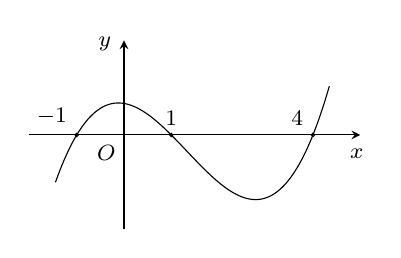
\begin{tikzpicture}[line cap=butt,line join=miter,>=stealth,font=\footnotesize,scale=.6]
            \tikzset{declare function={xmin=-2;xmax=5;ymin=-2;ymax=2;
                    f(\x)=1/6*((\x)^2-1)*((\x)-4);
                },
                smooth,samples=450
            }
            \draw[->] (xmin,0)--(xmax,0) node[shift={(-100:7pt)}]{$ x $};
            \draw[->] (0,ymin)--(0,ymax) node[shift={(190:7pt)}]{$ y $};
            \fill (0,0) node[shift={(-135:9pt)}]{$ O $};
            \draw (-1,0) circle (1pt) node[above left]{$-1$}
            (1,0) circle (1pt) node[above ]{$1$}
            (4,0) circle (1pt) node[above left]{$4$};
            \clip (xmin,ymin) rectangle (xmax,ymax);
            \draw  plot[domain=-1.45:4.35] (\x, {f(\x)});
    \end{tikzpicture}}
    %    \loigiai{
        %vì $f'(x) > 0,\forall x\in (-1;1)$ nên hàm số $y=f(x)$ đồng biến trên khoảng $(-1;1)$
        %    }
%    \dotlineEX{1}
\end{vd}

\begin{vd}%[2D1H1-2]
\immini[thm]
{
        Cho hàm số $y=f(x)$ có bảng biến thiên như sau\\
    Hàm số đã cho nghịch biến trên khoảng nào dưới đây?
    \choice
    {$(1 ;+\infty)$}
    {\True $(0 ; 1)$}
    {$(-1 ; 0)$}
    {$(0 ;+\infty)$}
}
{
    
\begin{tikzpicture}[>=stealth]
        \tkzTabInit[nocadre=true,lgt=1.5,espcl=1.7,deltacl=0.6]
        {$x$/.7, $f'(x)$/.7, $f(x)$/2}
        {$-\infty$, $-1$, $0$, $1$, $+\infty$}
        \tkzTabLine{, -, z, +, z, -, z, +,}
        \tkzTabVar{+/$+\infty$, -/$0$, +/$3$, -/$0$, +/$+\infty$}
    \end{tikzpicture}
}
    %    \loigiai{
        %        Dựa vào bảng biến thiên, hàm số đã cho nghịch biến trên các khoảng $(-\infty ;-1)$ và $(0 ; 1)$.
        %    }
\end{vd}
\begin{vd}%[2D1H2-1]
    Hàm số $f(x)=x^3-3x^2-9x+1$ đạt cực đại tại điểm
    \choice
    {\True $x=-1$}
    {$x=1$}
    {$x=3$}
    {$x=-3$}
    \loigiai{
        Ta có $f'(x)=3x^2-6x-9$, $f'(x)=0\Leftrightarrow\hoac{&x=-1\\
            &x=3.}$\\
        Ta có bảng biến thiên
        \begin{center}
            
\begin{tikzpicture}[>=stealth]
                \tkzTabInit[nocadre=true,lgt=1.5,espcl=2,deltacl=0.6]
                {$x$ /.7, $f’(x)$ /.7, $f(x)$ /2.5}
                {$-\infty$,$-1$,$3$,$+\infty$}
                \tkzTabLine{ ,+,$0$,-,$0$,+, }
                \tkzTabVar{-/$-\infty$,+/$6$,-/$-26$,+/$+\infty$}
            \end{tikzpicture}
        \end{center}
        Dựa vào bảng biến thiên, ta thấy hàm số đạt cực đại tại $x=-1$.
    }
\end{vd}
\begin{vd}%[2D1H2-1]
    Cho hàm số $y=7x^3+9x^2-3x-4$. Khẳng định nào sau đây là \textbf{sai}?
    \choice
    {Giá trị cực đại $y=1$}
    {Hàm số đạt cực tiểu tại $x=\dfrac{1}{7}$}
    {\True Giá trị cực tiểu $y=\dfrac{1}{7}$}
    {Hàm số đạt cực đại tại $x=-1$}
    \loigiai{
        Tập xác định $\mathbb{R}$.\\
        $y'=21x^2+18x-3$.\\
        $y'=0 \Leftrightarrow x=-1 \text{ hoặc } x=\dfrac{1}{7}$.\\
        Do đó, hàm số đạt cực đại tại $x=-1, y_{\text{CĐ}}=1$.\\
        Hàm số đạt cực tiểu tại $x=\dfrac{1}{7}, y_{\text{CT}}=- \dfrac{207}{49}$.
    }
\end{vd}
\begin{vd}%[2D1H2-1]
    Cho hàm số $y=\dfrac{x^2-4x+1}{x-4}$. Trong các khẳng định sau, khẳng định nào đúng?
    \choice
    {Hàm số đạt cực tiểu tại $x=3$, giá trị cực tiểu là $y=2$}
    {\True Hàm số đạt cực tiểu tại $x=5$, giá trị cực tiểu là $y=6$}
    {Hàm số đạt cực tiểu tại $x=3$, giá trị cực tiểu là $y=6$}
    {Hàm số đạt cực tiểu tại $x=5$, giá trị cực tiểu là $y=2$}
    \loigiai{
        Tập xác định $\mathscr{D}=\mathbb{R}\setminus \{4\}$.\\
        Ta có $y=x+\dfrac{1}{x-4} \Rightarrow y'=1-\dfrac{1}{(x-4)^2}=\dfrac{x^2-8x+15}{(x-4)^2}$;\\
        $y'=0 \Leftrightarrow x^2-8x+15=0 \Leftrightarrow \hoac{& x=3\\& x=5.}$\\
        Bảng biến thiên
        \begin{center}
            
\begin{tikzpicture}
                \tkzTabInit[nocadre=true,lgt=1.2,espcl=2.5,deltacl=0.6]
                {$x$ /0.6,$y'$ /0.6,$y$ /2}
                {$-\infty$,$3$,$4$,$5$,$+\infty$}
                \tkzTabLine{,+,$0$,-,d,-,$0$,+,}
                \tkzTabVar{-/$-\infty$,+/$2$,-D+/$-\infty$/$+\infty$,-/$6$,+/$+\infty$}
            \end{tikzpicture}
        \end{center}
        Vậy hàm số đạt cực tiểu tại $x=5$, giá trị cực tiểu là $y=6$.	
    }
\end{vd}

\begin{vd}[CHUYÊN KHTN Hà Nội L2]%[2D1N2-2]
\immini[thm]
{
        Cho hàm số $y=f(x)$ có bảng biến thiên như sau\\
    Điểm cực đại của hàm số đã cho là
    \choice
    {$21$}
    {$1$}
    {\True $-2$}
    {$-6$}
}
{
    
\begin{tikzpicture}
        \tkzTabInit[nocadre=true,lgt=1.5,espcl=2,deltacl=0.6]
        {$x$/0.7,$f'(x)$/0.7,$f(x)$/1.5}
        {$-\infty$,$-2$,$1$,$+\infty$}
        \tkzTabLine{,+,0,-,0,+,}
        \tkzTabVar{-/$-\infty$,+/$21$,-/$-6$,+/$+\infty$}
    \end{tikzpicture}
}
    %    \loigiai{
        %        Từ bảng biến thiên suy ra điểm cực đại của hàm số đã cho là $x=-2$.
        %    }
\end{vd}
\begin{vd}%[2D1N3-1]
    \immini[thm]{Cho hàm số $y=f(x)$ liên tục trên đoạn $[-1;3]$ và có đồ thị như hình vẽ bên. Giá trị lớn nhất của hàm số đã cho trên đoạn $[-1;2]$ bằng
        \choice
        {$3$}
        {$1$}
        {$-2$}
        {\True $2$}
    }
    {	\begin{tikzpicture}[scale=0.7, font=\footnotesize, line join=round, line cap=round, >=stealth]  
            \def\aa{-1} \def\bb{0} \def\cc{2}
            \draw[->] (-2,0)--(4,0)node[below right]{$x$};
            \draw[->] (0,-2.2)--(0,4)node[left]{$y$};
            \fill (0,0)circle (1pt) node[above left]{$O$};
            \draw[samples=150,smooth,domain=-1:2] plot(\x,{\aa*(\x)^2+\bb*\x+\cc});
            \draw (2,-2)--(3,3);
            \draw[dashed,thin] 
            (-1,0)node[below]{$-1$}--(-1,1)--(0,1) node[right]{$1$} (0,-2)node[left]{$-2$}--(2,-2)--(2,0)node[above]{$2$} (3,0)node[below]{$3$}--(3,3)--(0,3)node[left]{$3$};
            \fill (-1,1) circle (1pt);
            \fill (2,-2) circle (1pt);
            \fill (3,3) circle (1pt);
            \fill (0,2)circle (1pt) node[above left]{$2$};
        \end{tikzpicture}
    }
    %    \loigiai{
        %        Dựa vào đồ thị của hàm số ta có $\max\limits_{[-1;2]} y=2$.}
\end{vd}
\begin{vd}%[2D1H3-1]
    Giá trị lớn nhất của hàm số $f(x)=x^3-8x^2+16x-9$ trên đoạn $[1;3]$ là
    \choice
    {$\max\limits_{[1 ; 3]} f(x)=0$}
    {\True $\max\limits_{[1 ; 3]} f(x)=\dfrac{13}{27}$}
    {$\max\limits_{[1 ; 3]} f(x)=-6$}
    {$\max\limits_{[1 ; 3]} f(x)=5$}
    \loigiai{
        Hàm số $f(x)$ liên tục trên $[1 ; 3]$.\\
        Ta có $f'(x)=3x^2-16x+16$; $f'(x)=0 \Leftrightarrow \hoac{&x=4 \notin(1;3) \\&x=\dfrac{4}{3}  \in (1;3).}$\\
        $f(1)=0$; $f\left(\dfrac{4}{3}\right)=\dfrac{13}{27}$; $f(3)=-6$.\\
        Do đó $\max\limits_{[1;3]} f(x)=f\left(\dfrac{4}{3}\right)=\dfrac{13}{27}$.
    }
\end{vd}
\begin{vd}%[2D1H3-1]
    Tìm giá trị thực của tham số $a$ để hàm số $f(x)=-x^3-3 x^2+a$ có giá trị nhỏ nhất trên đoạn $[-1 ; 1]$ bằng 0.
    \choice
    {$a=2$}
    {$a=6$}
    {$a=0$}
    {\True $a=4$}
%    \loigiai{Xét hàm số $f(x)=-x^3-3 x^2+a$ trên $[-1 ; 1]$, có   $f'(x)=-3 x^2-6 x.$\\
%        Phương trình $f'(x)=0 \Leftrightarrow \heva{&-1 \leq x \leq 1 \\& -3 x^2-6 x=0} \Rightarrow x=0$.\\
%        Tính $f(-1)=-2+a ; f(0)=a ; f(1)=-4+a.$\\
%        Suy ra $\min \limits_{[-1: 1]} f(x)=f(1)=-4+a=0 \Rightarrow a=4$. 
%    }
\dotlineEX{1}
\end{vd}
\begin{vd}[TN2025-0101]%[2D1H4-1]
    \immini[thm]
 {
        Cho hàm số $y=\dfrac{ax+b}{cx+d}$ ($ac\ne 0$, $ad-bc\ne 0$) có đồ thị như hình đưới. Đường tiệm cận đứng của đồ thị hàm số đã cho có phương trình là
        \choice
        {$y=2$}
        {\True $x=-1$}
        {$y=-1$}
        {$x=2$}
    }
    {
        \begin{tikzpicture}[scale=0.6, font=\footnotesize,line join=round, line cap=round,>=stealth]
            \draw[->] (-4.5,0)--(0,0)node[below right]{$O$}--(3.5,0) node[below]{$x$};
            \draw[->] (0,-2)--(0,6) node [right]{$y$};
            \begin{scope}
                \clip (-4.5,-2) rectangle (3.5,6);
                \draw[smooth,samples=100] plot[domain=-0.75:3.5](\x,{(2*(\x)+1)/(\x+1)}) plot[domain=-4.5:-1.25](\x,{(2*(\x)+1)/(\x+1)});
            \end{scope}
            \draw[dashed](-1,6)--(-1,-2) (-4.5,2)--(3.5,2);
            \fill[black] 
            (0,0) circle(2pt) 
            (-1,0) node[below left]{$-1$} circle(1pt)
            (0,2) node[above right]{$2$} circle(1pt);
        \end{tikzpicture}
    }
    %    \loigiai{
        %        Dựa vào đồ thị hàm số, đường tiệm cận đứng của đồ thị hàm số đã cho có phương trình là $x=-1$.
        %    }
\end{vd}



\begin{vd}[CHUYÊN KHTN Hà Nội L2]%[2D1H4-1]
    Đường tiệm cận xiên của đồ thị hàm số $y=\dfrac{2x^2-x+2}{x+1}$ có phương trình là
    \choice
    {\True $y=2x-3$}
    {$y=2x+3$}
    {$y=x+1$}
    {$y=2x-1$}
    \loigiai{
        Tập xác định $\mathscr{D}=\mathbb{R}\setminus\{-1\}$.\\
        Ta có
        $a=\lim\limits_{x\to+\infty} \dfrac{f(x)}{x}=\lim\limits_{x\to+\infty} \dfrac{2x^2-x+2}{x^2+x}=2$; $b=\lim\limits_{x\to+\infty} [f(x)-ax]=\lim\limits_{x\to+\infty} \dfrac{-3x-2}{x+1}=-3$.\\
        Ta cũng có $\lim\limits_{x\to-\infty} \dfrac{f(x)}{x}=2$; $\lim\limits_{x\to-\infty} [f(x)-2x]=-3$.\\
        Do đó đồ thị hàm số có một tiệm cận xiên là đường thẳng $y=2x-3$.
    }
\end{vd}

\begin{vd}%[2D1H4-1]
    \immini[thm]{Cho hàm số $y=f(x)$ có bảng biến thiên. Tổng số đường tiệm cận của đồ thị hàm số $y= f(x)$ là
        \choice
        {$1$}
        {\True $2$}
        {$3$}
        {$4$}}
    {
\begin{tikzpicture}[>=stealth, scale=0.85]
            \tkzTabInit[nocadre=true,lgt=1,espcl=3,deltacl=0.5]{$x$/.7 ,$y'$/.7,$y$/1.5}
            {$-\infty$ , $1$ , $+\infty$}
            \tkzTabLine{ , - , d , - , }
            \tkzTabVar{+/$2$ ,-D+/$-\infty$/$+\infty$ , -/$2$}
    \end{tikzpicture}}
    %    \loigiai{
        %        Dựa vào bảng biến thiên ta có đồ thị hàm số có $2$ tiệm cận là $x=2$ tiệm cận đứng và $y=2$ tiệm cận ngang.
        %    }
\end{vd}
\begin{vd}%[2D1H5-1]
    \immini[thm]{ 
        Hàm số nào có đồ thị như hình bên?
        \choice[1]
        {$y=-x^3+3x-2$}
        {$y=-x^3-2$}
        {\True $y=-x^3+3x^2-2$}
        {$y=x^3-3x-2$}
    }{
        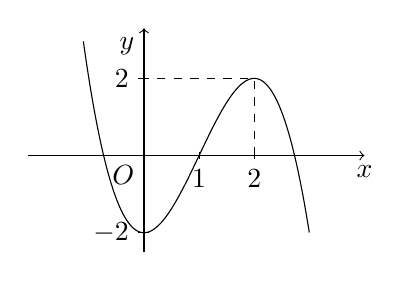
\begin{tikzpicture}[scale=.7,y=.7cm]
            \def\a{-1}
            \def\b{3}
            \def\c{0}
            \def\d{-2}
            \def\f(#1){\a*((#1)^3)+\b*((#1)^2)+\c*(#1)+\d}
            \def\xmin{-1.1}
            \def\xmax{3}
            \def\ymin{-1.5}
            \def\ymax{2.3}
            \draw[->] (\xmin-1,0)--(\xmax+1,0) node[below] { $x$};
            \draw[->] (0,\ymin-1)--(0,\ymax+1) node[below left] { $y$};
            \draw (0,0) node [below left] { $O$};
            \foreach \x in {1,2}\draw (\x,0.1)--(\x,-0.1) node [below] { $\x$};
            \foreach \y in {-2,2}\draw (0.1,\y)--(-0.1,\y) node [left] { $\y$};
            \draw[smooth,samples=200] plot[domain=\xmin:\xmax] (\x,{\f(\x)});
            \draw[dashed] (2,0)|-(0,2);
        \end{tikzpicture}
    }
    %    \loigiai{
        %        Dạng đồ thị hàm số đã cho là hàm số bậc ba có hệ số $a<0$ và có hai điểm cực trị $(0;-2)$ và $(2;2)$, đi qua điểm $(1;0)$.\\
        %        Do đó hàm số $y=-x^3+3x^2-2$ thỏa mãn đề bài.
        %    }
\end{vd}
\begin{vd}%[2D1H5-1]
    \immini
    {
        Đường cong dưới đây là đồ thị của hàm số nào?
        \choice[1]
        {$y=-x^3+x^2-2x+1$}
        {$y=\dfrac{x^2-x+3}{x-1}$}
        {\True $y=\dfrac{x^2-3x+6}{x-1}$}
        {$y=\dfrac{2x+3}{x-1}$}
    }
    {
        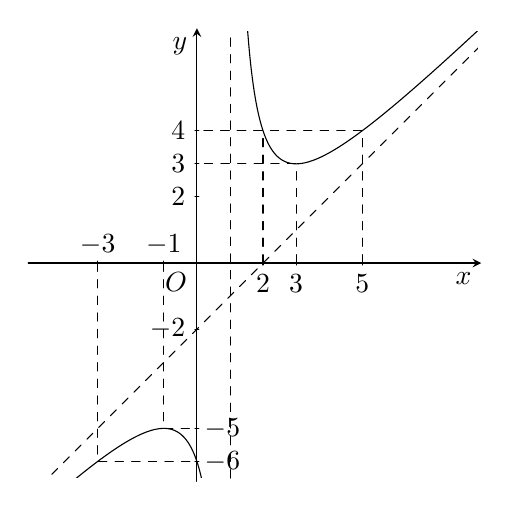
\begin{tikzpicture}[line join=round, line cap=round,>=stealth,scale=.7,x=.6cm,y=.6cm]
            \draw[->] (-5.1,0)--(8.6,0) node[below left] {$x$};
            \draw[->] (0,-6.6)--(0,7.1) node[below left] {$y$};
            \draw (0,0) node [below left] {$O$};
            \foreach \x/\nx in {2/2,3/3,5/5}
            \draw[thin] (\x,1pt)--(\x,-1pt) node [below] {$\nx$};
            \foreach \x/\nx in {-3/-3,-1/-1}
            \draw[thin] (\x,1pt)--(\x,-1pt) node [above] {$\nx$};
            \foreach \y/\ny in {-2/-2,2/2,3/3,4/4}
            \draw[thin] (1pt,\y)--(-1pt,\y) node [left] {$\ny$};
            \foreach \y/\ny in {-6/-6,-5/-5}
            \draw[thin] (1pt,\y)--(-1pt,\y) node [right] {$\ny$};
            \draw[dashed](-3,0)--(-3,-6)--(0,-6);
            \draw[dashed,](-1,0)--(-1,-5)--(0,-5);
            \draw[dashed,](2,0)--(2,4)--(0,4);
            \draw[dashed,](3,0)--(3,3)--(0,3);
            \draw[dashed,](5,0)--(5,4)--(0,4);
            \draw[dashed] (1.01,-6.5)--(1.01,7);
            \begin{scope}
                \clip (-5,-6.5) rectangle (8.5,7);
                \draw[samples=200,domain=-5:0.99,smooth,variable=\x] plot (\x,{(1*((\x)^2)+-3*(\x)+6)/(1*(\x)+-1)});
                \draw[samples=200,domain=1.01:8.5,smooth,variable=\x] plot (\x,{(1*((\x)^2)+-3*(\x)+6)/(1*(\x)+-1)});
                \draw[dashed] (-5.1,-7.1)--(8.6,6.6);
            \end{scope}
        \end{tikzpicture}
    }
%    \loigiai{
%        Đồ thị hàm số có dạng $y=\dfrac{ax^2+bx+c}{mx+n}$, có tiệm cận đứng $x=1$ và tiệm cận xiên $y=x-2$, đi qua các điểm $A(3;3)$, $B(5;4)$, $C(-1;-5)$.\\
%        Vậy $y=\dfrac{x^2-3x+6}{x-1}$.
%    }
\dotlineEX{3}
\end{vd}

\begin{vd}%[2D1H5-1]
    \immini[thm]{ 
        Đường cong ở hình bên là đồ thị của hàm số nào sau đây?
        \choice[1]
        {$y=\dfrac{x+1}{x-1}$}
        {$y=\dfrac{-x+1}{x+1}$}
        {$y=\dfrac{x-1}{x+1}$}
        {\True $y=\dfrac{-x}{x+1}$}
    }{
        \begin{tikzpicture}[scale=.7]
            
            
            \def\a{-1}
            \def\b{0}
            \def\c{1}
            \def\d{1}
            \def\f(#1){(\a*(#1)+\b)/(\c*(#1)+\d)}
            \def\xmin{-4}
            \def\xmax{2}
            \def\ymin{-4}
            \def\ymax{2}
            \def\m{-\d/\c} %Điểm cận để vẽ đồ thị 
            \def\n{0.3} %hãy thay đổi để biết cụ thể
            \draw[->] (\xmin-.5,0)--(\xmax+.5,0) node[below] { $x$};
            \draw[->] (0,\ymin-.5)--(0,\ymax+.5) node[left] { $y$};
            \draw (0,0) node [below left] { $O$};
            \foreach \x in {-2,-1}\draw (\x,0.1)--(\x,-0.1) node [below left] { $\x$};
            \foreach \y in {-2,-1}\draw (0.1,\y)--(-0.1,\y) node [below right] { $\y$};
            \draw[dashed] (-\d/\c,\ymin)--(-\d/\c,\ymax);
            \draw[dashed] (\xmin,\a/\c)--(\xmax,\a/\c);
            \draw[smooth,samples=200] plot[domain=\xmin:{\m-\n}] (\x,{\f(\x)});
            \draw[smooth,samples=200] plot[domain={\m+\n}:\xmax] (\x,{\f(\x)});
            \draw[dashed] (-2,0)|-(0,-2);
        \end{tikzpicture}
    }
%    
%    \loigiai{
%        Dạng đồ thị hàm số đã cho là hàm số $y=\dfrac{ax+b}{cx+d}$ có tiệm cận đứng $x=-1$, tiệm cận ngang $y=-1$ và đi qua điểm $(0;0)$. Suy ra $y=\dfrac{-x}{x+1}$
%    }
\end{vd}

\begin{vd}%[2-D1B4-SO-12-2425]%[VN-MT-7, VM22]%[2D1H5-3]
    Cho hàm số $y=f(x)$ có bảng biến thiên như sau:\\
    \centerline{
        
\begin{tikzpicture}
            \tkzTabInit[nocadre=true,lgt=1.2,espcl=3]
            {$x$/0.7,$f'(x)$/0.7,$f(x)$/2}
            {$-\infty$,$1$,$2$,$+\infty$}
            \tkzTabLine{,+,$0$,-,$0$,+,}
            \tkzTabVar{-/$-\infty$,+/$4$,-/$0$,+/$+\infty$}
        \end{tikzpicture}
    }
    Phương trình $f(x)=3$ có bao nhiêu nghiệm?
    \choice
    {vô nghiệm}
    {$1$}
    {$2$}
    {\True $3$}
    \loigiai{
        Từ bảng biến thiên ta thấy phương trình $f(x)=3$ có $3$ nghiệm.
    }
\end{vd}
\begin{vd}%[2D1H5-3]
    Cho hàm số $y=f(x)$ có bảng biến thiên bên dưới.
    \begin{center}
        
\begin{tikzpicture}
            \tkzTabInit[nocadre=true,lgt=1.5,espcl=2.5,deltacl=0.5]
            {$x$/.6 ,$y'$/.6,$y$/2}
            {$-\infty$ , $-1$ , $1$ , $+\infty$}
            \tkzTabLine{ , + , $0$ , - , $0$ , + , }
            \tkzTabVar{-/$1$ , +/$3$ , -/$\dfrac{1}{3}$ , +/$1$}
        \end{tikzpicture}
    \end{center}
    Số nghiệm của $2f^2(x)-3f(x)+1=0$ là
    \choice
    {$6$ nghiệm}
    {$0$ nghiệm}
    {\True $3$ nghiệm}
    {$2$ nghiệm}
    \loigiai{
        Ta có $2f^2(x)-3f(x)+1=0\Leftrightarrow \hoac{&f(x)=1\\&f(x)=\dfrac{1}{2}.}$\\
        Dựa vào bảng biến thiên, đường thẳng $y=1$ cắt đồ thị hàm số tại $1$ điểm nên phương trình $f(x)=1$ có $1$ nghiệm, còn đường thẳng $y=\dfrac{1}{2}$ cắt đồ thị hàm số tại $2$ điểm nên phương trình $f(x)=\dfrac{1}{2}$ có $2$ nghiệm. Rõ ràng các nghiệm này đôi một phân biệt.\\
        Vậy phương trình đã cho có $3$ nghiệm.
    }
\end{vd}
\begin{vd}%[2-D1B4-SO-11-2425]%[VN-MT-7, Nguyễn Tuấn]%[2D1H5-4]
    Cho hàm số $y=\dfrac{x^2+2x-1}{x-1}$ và $y=2x-7$. Hai đồ thị hàm số cắt nhau tại hai điểm thì tổng hoành độ hai giao điểm bằng
    \choice
    {$7$}
    {$5$}
    {$8$}
    {\True $11$}
    \loigiai{
        Phương trình hoành độ giao điểm của hai đồ thị \[\dfrac{x^2+2x-1}{x-1}=2x-7 \Leftrightarrow\heva{&x \ne 1 \\& x^2-11x+8=0.}\]
        Suy ra, tổng hoành độ của hai giao điểm là $x_1+x_2=11$.
    }
    
\end{vd}
\begin{vd}%[2D1H5-5]
    \immini[thm]{Cho hàm số $f(x)$ có đồ thị hàm số $y=f'(x)$ như hình bên. Mệnh đề nào dưới đây đúng?
        \choice
        {$f(-4)>f(-2)$}
        {Hàm số đã cho có hai điểm cực trị}
        {Hàm số đã cho nghịch biến trên khoảng $(-3;0)$}
        {\True $f(0)>f(3)$}
    }{
        \begin{tikzpicture}[>=stealth,scale=0.7,y=.8cm]
            \def\a{0.104} % Hệ số a phải khác 0
            \def\b{0.3125}
            \def\c{-1.0416}
            \def\d{-2.5}
            \draw[->] (-5,0) -- (5,0)node[below]{$x$};
            \draw[->] (0,-3) -- (0,2.7) node[left] {$y$};
            \draw (0,0)node[below left]{$O$};
            \clip (-5,-3.5)rectangle(5,3);
            \fill (-2,0) circle (1pt) node[ above ]{$-2$};
            \fill (-4,0) circle (1pt) node[ below right]{$-4$};
            \fill (3,0) circle (1pt) node[ above right ]{$3$};
            \draw[samples=150,smooth,domain=-5:3.5] plot(\x,{\a*(\x)^3+(\b)*(\x)^2+(\c)*\x+(\d)});
        \end{tikzpicture}
    }
%    
%    \loigiai{
%        Dựa vào đồ thị hàm số của $y=f'(x)$, ta thấy với $x\in(0;3)$ thì $f'(x) <0$.\\ $\Rightarrow$ Hàm số nghịch biến trên khoảng $(0;3)$.\\
%        Suy ra $f(0)>f(3)$.		
%    }
\end{vd}
\begin{vd}%[Dự Án Bài Giảng 12 4 in 1, Lê Văn Toàn]%[2D1H5-6]
    Hàm số $ f(x)=x^3-3x^2+4$ có đồ thị $(C) $. Viết phương trình tiếp tuyến với $(C)$ tại điểm $A$ có hoành độ $x_A=1 $.
    \choice
    {\True $ y=-3x+5 $}
    {$ y=-5x+3 $}
    {$ y=3x-5 $}
    {$ y=5x-3 $}
    \loigiai{
        Ta có $ y'=3x^2-6x $.\\
        Với $ x_A=1$, ta có $y_A=2$ và $ y'\left(x_A\right)=y'(1)=-3 $.\\
        Vậy phương trình tiếp tuyến tại $A$ là $ y=-3(x-1)+2 \Leftrightarrow y=-3x+5 $.
    }
\end{vd}
\begin{vd}%[2D1V5-8]
    Một vật chuyển động theo quy luật $s=-2t^3+24t^2+9t-3$ với $ t$ là khoảng thời gian tính từ lúc bắt đầu chuyển động và $ s$ là quãng đường vật đi được trong khoảng thời gian đó. Hỏi trong khoảng thời gian $10$ giây, kể từ lúc bắt đầu chuyển động, vận tốc lớn nhất của vật đạt được bằng bao nhiêu?
    \choice
    {$289$ (m/s)}
    {\True $105$ (m/s)}
    {$111$ (m/s)}
    {$487$ (m/s)}
    \loigiai{Ta có $ v(t)=s'=-6t^2+48t+9$. Xét hàm số $ v(t)=-6t^2+48t+9$, $ t\in[0;10]$.\\
        Ta có $v'(t)=-12t+48=0\Leftrightarrow t=4$ (nhận).\\
        Ta có $v(0)=9$, $v(4)=105$, $v(10)=-111$.\\
        Suy ra $\max\limits_{t\in[0;10]}v(t)=v(4)=105$.}
        \dotlineEX{3}
\end{vd}
\begin{vd}%[2D1V2-7] 
    Một xưởng in có  $8$  máy in, mỗi máy in được  $4\,000$  bản in khổ giấy A$4$ trong một giờ. Chi phí để bảo trì, vận hành một máy trong mỗi lần in là  $50\,000$  đồng. Chi phí in ấn của $n$ máy chạy trong một giờ là $20(3n+5)$ nghìn đồng. Hỏi nếu in  $50\,000$  bản in khổ giấy A$4$ thì phải sử dụng bao nhiêu máy để thu được nhiều lãi nhất? 
    \choice
    {$4$ máy}
    {$7$ máy}
    {$6$ máy}
    {\True  $5$ máy}
    \loigiai{
        Gọi số giờ cần in là $x$ thì $n$ máy in được $4000 \cdot n \cdot x$ bản in trong $x$ giờ.\\
        Ta có $4000\cdot n \cdot x=50000 \Rightarrow n \cdot x=\dfrac{25}{2}$.\\
        Chi phí in ấn của $n$ máy chạy trong $x$ giờ là $20x(3n+5)$ nghìn đồng.\\
        Chi phí để bảo trì $n$ máy là $50n$ nghìn đồng.\\
        Tổng chi phí là $f(n)=20x(3n+5)+50n=60x n+100x+50n=750+\dfrac{1250}{n}+50n$.\\
        Ta có
        $f'(n)=-\dfrac{1250}{n^2}+50$, $f'(n)=0 \Leftrightarrow n=5$.\\
        Bảng biến thiên
        \begin{center}
            
\begin{tikzpicture}[scale=1, font=\footnotesize, line join=round, line cap=round, >=stealth]
                \tkzTabInit[nocadre=false,lgt=1,espcl=2,deltacl=0.5]
                {$n$/.7 ,$f'(n)$/.7,$f(n)$/2}
                {$1$ , $5$ , $8$}
                \tkzTabLine{ , - , $0$ , + , }
                \tkzTabVar{+/ , -/$f(5)$ , +/}
            \end{tikzpicture}
        \end{center}
        Để thu được tiền lãi cao nhất thì cần chi phí thấp nhất, vậy $n=5$ thỏa mãn yêu cầu bài toán.
    }
    \dotlineEX{6}
\end{vd}
\begin{vd}%[2D1V3-6]
    Một công ty bất động sản có $40$ căn hộ cho thuê. Biết rằng nếu cho thuê mỗi căn hộ với giá $3\,000\,00$ đồng một tháng thì mọi căn hộ đều có người thuê và cứ tăng thêm giá mỗi căn hộ $100\,000$ đồng một tháng (theo quy định trong hợp đồng) thì sẽ có một căn hộ bị bỏ trống. Hỏi muốn có thu nhập cao nhất thì công ty đó phải cho thuê mỗi căn hộ với giá bao nhiêu một tháng?
    \choice
    {\True $3\,500\,000$ đồng}
    {$4\,000\,000$ đồng}
    {$3\,700.000$ đồng}
    {$3\,900\,000$ đồng}
    \loigiai{
        Gọi $x$ là số căn hộ bị bỏ trống $\left(0 \le x \le 40\right)$.\\
        Vậy giá cho thuê một căn phòng là $3+0{,}1x$ (triệu đồng).\\
        Số căn hộ cho thuê là $40-x$. \\
        Số tiền thu được là 
        $$T=(40-x) \cdot (3+0{,}1x)=-0{,}1x^2+x+120 \Rightarrow T'=-0{,}2x+1 \Rightarrow T'=0 \Rightarrow x=5.$$
        Ta có bảng biến thiên
        \begin{center}
            
\begin{tikzpicture}
                \tkzTabInit[espcl=2.5,lgt=1.5]
                {$x$/0.7,$T'$/0.7,$T$/2.1}
                {$0$,$5$,$40$}
                \tkzTabLine{,+,0,-,}
                \tkzTabVar{-/$ $,+/$ 3\,500\,000 $,-/$ $}
            \end{tikzpicture}
        \end{center}
        Vậy $T$ đạt giá trị lớn nhất khi $x=5$, khi đó giá thuê một căn phòng là $3\,500\,000$ đồng.
    }
    \dotlineEX{4}
\end{vd}
\begin{vd}%[2D1V3-6]
    Một người bán buôn Thanh Long Đỏ nhận thấy rằng: Nếu bán với giá $20\,000$ đồng/kg thì mỗi tuần có $90$ khách đến mua và mỗi khách mua trung bình $60$ kg. Cứ tăng giá $2\,000$ đồng/kg thì số khách mua hàng tuần giảm đi $1$ và khi đó mỗi khách lại mua ít hơn mức trung bình $5$ kg, và như vậy cứ giảm giá $2\,000$ đồng/kg thì số khách mua hàng tuần tăng thêm $1$ và khi đó mỗi khách lại mua nhiều hơn mức trung bình $5$ kg. Hỏi người đó phải bán với giá mỗi kg là bao nhiêu để lợi nhuận thu được hàng tuần là lớn nhất, biết rằng người đó phải nộp tổng các loại thuế là $2\,200$ đồng/kg (kết quả làm tròn đến hàng nghìn).
    \choice
    {$16\,000$ đ}
    {$12\,000$ đ}
    {$24\,000$ đ}
    {\True $22\,000$ đ}
    \loigiai{
        Giả sử giá bán thay đổi $x$ lần, mỗi lần thay đổi $2\,000$ đồng ($x\in\mathbb{Z}$, $x>0$ là tăng giá, $x<0$ là giảm giá).\\
        Theo thực tế thì $-10<x<45$ (giá bán trên $0$ đồng và còn ít nhất một khách).\\
        Tổng tiền thu được sau khi thay đổi là \\
        $T=(90-x)(60-5x)(20+2x-2{,}2)=10x^3-931x^2+1772x+96120$.\\
        Xét hàm số $T(x)=10x^3-931x^2+1772x+96120$.\\
        Bài toán trở thành tìm GTLN của $T(x)$ với $x\geq 20\,000$.\\
        Ta có $T'(x)=30(x^2-62\text{,}0667x+57\text{,}4)$.\\
        $T'=0\Leftrightarrow \hoac{&x\approx 1\\&x\approx 61.}$\\
        Bảng biến thiên của $T(x)$
        \begin{center}
            \begin{tikzpicture}
                \tkzTabInit[lgt=1.2,espcl=3]
                {$x$  /1.2, $T'(x)$ /1.2,$T(x)$  /2.0}
                {$-10$ , $1$, $45$}
                \tkzTabLine{,+,z,-,}
                \tkzTabVar{-/,+/$T_\text{CĐ}$, -/}
            \end{tikzpicture}
        \end{center}
        Dựa vào bảng biến thiên suy ra $T$ lớn nhất khi $x=1$, tức là ta chỉ tăng giá một lần.\\
        Vậy giá bán đưa ra để lợi nhuận cao nhất là $22\,000$.
    }
    \dotlineEX{3}
\end{vd}
\begin{vd}%[2D1V3-6]
    Một người bán gạo muốn đóng một thùng tôn đựng gạo có thể tích không đổi bằng $10\mathrm{~m}^3$. Thùng tôn là hình hộp chữ nhật có chiều dài đáy bằng hai lần chiều rộng và không có nắp. Trên thị trường giá tôn làm đáy thùng là $75.000$ đồng/m$^2$ và giá tôn làm thành xung quanh thùng là $55.000$ đồng/m$^2$. Tính chi phí thấp nhất để làm thùng đựng gạo. (Làm tròn đến hàng nghìn)
    \choice
    {$1.418.000$ đồng}
    {$1.403.000$ đồng}
    {\True$1.402.000$ đồng}
    { $1.417.000$ đồng}
    \loigiai{		
        Gọi $x$ là chiều rộng của đáy thùng, $x > 0$, đơn vị m.\\
        Suy ra chiều dài của đáy thùng là $2 x$ (m).\\
        Ta có thể tích của thùng tôn là $V=x\cdot2x\cdot h=10\Rightarrow h=\dfrac{5}{x^2}$.\\
        Chi phí làm đáy thùng là $2x^2\cdot75=150x^2$ (nghìn đồng).\\
        Chi phí làm diện tích xung quanh là $\left(2\cdot x \cdot \dfrac{5}{x^2}+2\cdot 2x \cdot \dfrac{5}{x^2}\right) \cdot 55=\dfrac{1650}{x}$ (nghìn đồng).\\
        Suy ra chi phí làm thùng là $: T=150x^2+\dfrac{1650}{x}$ (đơn vị nghìn đồng).\\
        Xét hàm số $T=150x^2+\dfrac{1650}{x}$ , với $x > 0$.\\
        Ta có $T'(x)=300x-\dfrac{1650}{x^2}; T'(x)=0\Leftrightarrow x=\sqrt[3]{\dfrac{11}{2}}$.\\
        Bảng biến thiên của $T(x)$ trên $(0,+\infty)$:
        \begin{center}
            
\begin{tikzpicture}
                \tkzTabInit[nocadre=false,lgt=1.2,espcl=2,deltacl=0.6]
                {$t$/1,$T'(x)$/0.7,$T(x)$/2}
                {$0$,$\sqrt[3]{\frac{11}{2}}$,$+\infty$}
                \tkzTabLine{d,-,0,+,}
                \tkzTabVar{D+/$+\infty$,-/$1402$,+/$+\infty$}
            \end{tikzpicture}
        \end{center}
        \noindent	Dựa vào bảng biến thiên $T(x)$ đạt giá trị nhỏ nhất tại $x=\sqrt[3]{\dfrac{11}{2}}$.\\
        Vậy chi phí ít nhất bằng $T=150\sqrt[3]{\dfrac{11}{2}}^2+\dfrac{1650}{\sqrt[3]{\dfrac{11}{2}}}=1402$ (nghìn đồng).
    }
    \dotlineEX{3}
\end{vd}
\begin{vd}%[2D1V3-6] 
    \immini[thm]{Cho hình vuông $ABCD$ có cạnh bằng $4$,chính giữa có một hình vuông đồng tâm với $ABCD$. Biết rằng bốn tam giác là bốn tam giác cân. Hỏi tổng diện tích của hình vuông ở giữa và bốn tam giác cân nhỏ nhất bằng bao nhiêu?
        \choice
        { $\dfrac{19}{3}$}
        { $\dfrac{17}{3}$}
        {\True  $\dfrac{16}{3}$}
        { $\dfrac{14}{3}$}
    }{
        \begin{tikzpicture}[scale=0.5, font=\footnotesize, line join=round, line cap=round,>=stealth]
            %Gán tọa độ.
            \coordinate (A) at (0,6);
            \coordinate (B) at (6,6);
            \coordinate (C) at (6,0);
            \coordinate (D) at (0,0);
            %Trục Oxy.
            %Giới hạn đồ thị.
            \draw[fill=orange] (3,4)--(2,3)--(3,2)--(4,3)--cycle;
            \draw[fill=blue] (0,5)--(2,3)--(0,1)--cycle;	
            \draw[fill=blue!50] (4,3)--(6,1)--(6,5)--cycle;	
            \draw[fill=yellow] (1,0)--(3,2)--(5,0)--cycle;	
            \draw[fill=pink] (1,6)--(3,4)--(5,6)--cycle;	
            \draw (D) rectangle (B);
            \foreach \x/\y in {A/180, B/0, C/00, D/180}{\fill (\x) circle(1.2pt) ($(\x)+(\y:0.5cm)$) node{$\x$};}
        \end{tikzpicture}
    }
    \loigiai{
        \begin{center}
            \begin{tikzpicture}[scale=0.5, font=\footnotesize, line join=round, line cap=round,>=stealth]
                %Gán tọa độ.
                \coordinate (A) at (0,6);
                \coordinate (B) at (6,6);
                \coordinate (C) at (6,0);
                \coordinate (D) at (0,0);
                \coordinate (M) at (1,6);
                \coordinate (E) at (5,6);
                \coordinate (N) at (0,5);
                %Trục Oxy.
                %Giới hạn đồ thị.
                \draw[fill=orange] (3,4)--(2,3)--(3,2)--(4,3)--cycle;
                \draw[fill=blue] (0,5)--(2,3)--(0,1)--cycle;	
                \draw[fill=blue!50] (4,3)--(6,1)--(6,5)--cycle;	
                \draw[fill=yellow] (1,0)--(3,2)--(5,0)--cycle;	
                \draw[fill=pink] (1,6)--(3,4)--(5,6)--cycle;	
                \draw (D) rectangle (B);
                \foreach \x/\y in {A/180, B/0, C/00, D/180, M/90, E/90, N/180}{\fill (\x) circle(1.2pt) ($(\x)+(\y:0.5cm)$) node{$\x$};}
            \end{tikzpicture}
        \end{center}
        Đặt $AM=x$, $( 0<x<4 )$.\\
        Suy ra $ME=4-2x$.
        Ta có \begin{align*}
            &\, 2MQ^2={( 4-2x )}^2 \\ 
            \Leftrightarrow&\, MQ^2=2(2-x)^2 \\ 
            \Leftrightarrow&\, MQ=\sqrt{2(2-x)}.
        \end{align*}
        Gọi $S$ tổng diện tích của hình vuông ở giữa và bốn tam giác cân nhỏ
        $$S=4\cdot\dfrac{MQ^2}{2}+PQ^2=2MQ^2+MN^2=(4-2x)^2+\left(x\sqrt{2}\right)^2=6x^2-16x+16.$$
        Ta có $S'=12x-16=0\Leftrightarrow x=\dfrac{4}{3}$.\\
        Bảng biến thiên
        \begin{center}
            
\begin{tikzpicture}[scale=1, font=\footnotesize]
                \tkzTabInit[nocadre=false, lgt=1.2, espcl=2, deltacl=0.6]
                {$x$/0.8,$S'$/0.6,$S$/2}
                {$-\infty$,$\dfrac{4}{3}$,$+\infty$};
                \tkzTabLine{,-,$0$,+,};
                \tkzTabVar{+/$+\infty$,-/$\dfrac{16}{3}$,+/$+\infty$};
            \end{tikzpicture}
        \end{center}
        Vậy $\min S=\dfrac{16}{3}$.} 
        \dotlineEX{3}
\end{vd}
\begin{vd}%[TEX NBV]%[Đỗ Minh Phúc]%[2D1V3-6]
    Ông A dự định sử dụng hết $6{,}7$ m$^2$ kính để làm một bể cá bằng kính có dạng hình hộp chữ nhật không nắp, chiều dài gấp đôi chiều rộng (các mối ghép có kích thước không đáng kể). Bể cá có dung tích lớn nhất bằng bao nhiêu (kết quả làm tròn đến hàng phần trăm)?
    \choice
    {\True $1{,}57$ cm$^3$}
    {$1{,}11$ cm$^3$}
    {$1{,}23$ cm$^3$}
    {$2{,}48$ cm$^3$}
    \loigiai{
        Gọi $x$ là chiều rộng, ta có chiều dài là $2x$ (điều kiện $x>0$).\\
        Do diện tích đáy và các mặt bên là $6{,}7$ m$^2$ nên có chiều cao $h=\dfrac{6{,}7-2x^2}{6x}$, ta có $h>0$ nên $x<\sqrt{\dfrac{6{,}7}{2}}$.\\
        Thể tích bể cá là $V(x)=\dfrac{6{,}7x-2x^3}{3}$ và $V'(x)=\dfrac{6{,}7-6x^2}{3}=0 \Leftrightarrow x=\sqrt{\dfrac{6{,}7}{6}}$ (do $x>0$).\\
        Bảng biến thiên
        \begin{center}
            
\begin{tikzpicture}
                \tkzTabInit[nocadre,lgt=1.2,espcl=2.5,deltacl=0.6]
                {$x$/1,$V'(x)$/0.7,$V(x)$/2}{$0$,$\sqrt{\dfrac{6{,}7}{6}}$,$\sqrt{\dfrac{6{,}7}{2}}$}
                \tkzTabLine{,+,0,-,}
                \tkzTabVar{-/$0$,+/$1{,}57$,-/$0$}
            \end{tikzpicture}
        \end{center}	
        Bể cá có dung tích lớn nhất bằng $1{,}57$ cm$^3$.
    }
    \dotlineEX{3}
\end{vd}
\begin{vd}%[2D1V3-6]
    Sau khi phát hiện một bệnh dịch, các chuyên gia y tế ước tính số người nhiễm bệnh kể từ ngày xuất hiện bệnh nhân đầu tiên đến ngày thứ $t$ là  $f(t) =15t^2 -t^3$ (theo kết quả khảo sát các năm vừa qua). Nếu xem $f'(t)$ là tốc độ truyền bệnh (người/ngày) tại thời điểm $t$ thì vào ngày mà tốc độ truyền bệnh lớn nhất, số người nhiễm bệnh là bao nhiêu?
    \choice
    {$500$}
    {\True $250$}
    {$600$}
    {$75$}
    \loigiai{
        Ta có $f'(t) = -3t^2 +30t$ và $f''(t) = -6t + 30$.\\
        Lại có $f''(t) =0 \Leftrightarrow t=5$.\\
        Bảng biến thiên của hàm số $f'(t)$ ($t>0$).
        \begin{center}
            
\begin{tikzpicture}
                \tkzTabInit[lgt=1.2,espcl=2.5]
                {$t$  /1.0, $f''(t)$ /1.0,$f'(t)$ /2.2}
                {$0$ , $5$ ,$+\infty$}
                \tkzTabLine{,+,0,-,}
                \tkzTabVar{-/$0$ ,+/$75$, -/$-\infty$}
            \end{tikzpicture}
        \end{center}
        Vậy vào ngày tốc độ truyền bệnh lớn nhất, số người nhiễm bệnh là $f(5)=250$ người.
    }
    \dotlineEX{4}
\end{vd}
\Closesolutionfile{ans}
\subsection{\btrl}
\Opensolutionfile{ans}[ans/DA-CD1-BTRL]
\begin{ex}[TN2025-0101]%[2D1H3-1]
    Cho hàm số $f(x)=x^3-12x-8$.
    \choiceTF
    {\True Hàm số đã cho có đạo hàm là $f'(x)=3x^2-12$}
    {Phương trình $f'(x)=0$ có tập nghiệm là $S=\{2\}$}
    {$f(2)=24$}
    {Giá trị lớn nhất của hàm số $f(x)$ trên đoạn $[-3;3]$ bằng $24$}
    \loigiai
    {Hàm số $f(x)$ xác định và liên tục trên $\mathbb{R}$.
        \begin{itemchoice}
            \itemch Ta có $f'(x)=3x^2-12$.
            \itemch Phương trình $f'(x)=0 \Leftrightarrow 3x^2-12=0 \Leftrightarrow x=\pm 2$ nên có tập nghiệm là $S=\{-2;2\}$.
            \itemch Dễ thấy $f(2)=2^3-12\cdot 2-8 =-24$.
            \itemch	Bảng biến thiên của hàm số $f(x)$ trên đoạn $[-3;3]$ như sau
            \begin{center}
                
\begin{tikzpicture}
                    \tkzTabInit[nocadre=false,lgt=1.5,espcl=3.5,deltacl=0.6]
                    {$x$ /0.6,$f'(x)$ /0.6,$f(x)$ /2}
                    {$-3$,$-2$,$2$,$3$}
                    \tkzTabLine{,+,$0$,-,$0$,+,}
                    \tkzTabVar{-/$1$,+/$8$,-/$-24$,+/$-17$}
                \end{tikzpicture}
            \end{center}
            Vậy giá trị lớn nhất của hàm số $f(x)$ trên đoạn $[-3;3]$ là $8$.
    \end{itemchoice}}
\dotlineEX{2}
\end{ex}
\begin{ex}[CHUYÊ LÊ KHIẾT]%[2D1H3-1]
    Cho hàm số $y=f(x)=2\sin x+x$.
    \choiceTF
    {\True $f(0)=0$; $f(\pi)=\pi$} 
    {Đạo hàm của hàm số đã cho là $f'(x)=-2\cos x+1$} 
    {Số nghiệm của phương trình $f'(x)=0$ trên đoạn $[0; 3 \pi]$ là $6$} 
    {\True Giá trị lớn nhất của $f(x)$ trên đoạn $[0; \pi]$ là $\dfrac{2\pi}{3}+\sqrt{3}$}
    \loigiai{
        \begin{itemchoice}
            \itemch Ta có $\heva{&f(0)=2 \sin 0+0=0 \\&f(\pi)=2 \sin \pi+\pi=\pi.}$
            \itemch Ta có $y=f(x)=2 \sin x+x \Rightarrow f'(x)=2 \cos x+1$.
            \itemch Xét trên đoạn $[0 ; 3 \pi]$, ta có\\
            $f'(x)=0 \Leftrightarrow 2 \cos x+1=0 \Leftrightarrow \cos x=-\dfrac{1}{2} \Leftrightarrow x=\pm \dfrac{2 \pi}{3}+k 2 \pi \quad (k \in \mathbb{Z})$.\\
            Vì $0 \leq x \leq 3 \pi$ nên ta tìm các giá trị $k$ nguyên thỏa mãn:
            \begin{itemize}
                \item $0 \le \dfrac{2\pi}{3} + k2\pi \le 3\pi \Leftrightarrow -\dfrac{2\pi}{3} \le k2\pi \le \dfrac{7\pi}{3} \Leftrightarrow -\dfrac{1}{3} \le k \le \dfrac{7}{6}$.\\
                Suy ra $k \in \{0, 1\}$, ta được nghiệm $x=\dfrac{2\pi}{3}$ và $x=\dfrac{8\pi}{3}$.
                \item $0 \le -\dfrac{2\pi}{3} + k2\pi \le 3\pi \Leftrightarrow \dfrac{2\pi}{3} \le k2\pi \le \dfrac{11\pi}{3} \Leftrightarrow \dfrac{1}{3} \le k \le \dfrac{11}{6}$.\\
                Suy ra $k=1$, ta được nghiệm $x=\dfrac{4\pi}{3}$.
            \end{itemize}
            Vậy phương trình $f'(x)=0$ có $3$ nghiệm $x \in\left\{\dfrac{2 \pi}{3} ; \dfrac{4 \pi}{3} ; \dfrac{8 \pi}{3}\right\}$ trên đoạn $[0 ; 3 \pi]$.
            \itemch Xét trên đoạn $[0 ; \pi]$.\\
            Ta có $f'(x)=0 \Leftrightarrow 2 \cos x+1=0 \Leftrightarrow \cos x=-\dfrac{1}{2}x=\pm \dfrac{2 \pi}{3}+k 2 \pi$.\\
            Vì $0 \leq x \leq \pi$ nên $x=\dfrac{2 \pi}{3}$.\\
            Ta có
            $\heva{&f(0)=0\\&f\left(\dfrac{2 \pi}{3}\right)=\sqrt{3}+\dfrac{2 \pi}{3}\\&f(\pi)=\pi.}$\\
            Vậy giá trị lớn nhất của $f(x)$ trên đoạn $[0 ; \pi]$ là $\dfrac{2 \pi}{3}+\sqrt{3}$ khi $x=\dfrac{2\pi}{3}$.
        \end{itemchoice}
    }
    \dotlineEX{2}
\end{ex}
\begin{ex}[SỞ TUYÊN QUANG]%[1D7V2-1]
    Cho hàm số $f(x)=\sin x+\cos x$.
    \choiceTF
    {\True Đạo hàm của hàm số đã cho là $f'(x)=\cos x-\sin x$}
    {Giả sử $\sin x+\cos x=\dfrac{\sqrt{2}}{2}$ khi đó $\sin x \cdot \cos x=\dfrac{1}{4}$}
    {Giá trị lớn nhất của hàm số $f(x)$ trên đoạn $\left[0; \dfrac{3\pi}{4}\right]$ là bằng $a \sqrt{b}$, với $a$, $b$ là các số nguyên dương. Khi đó $b-a=2$}
    {\True Tổng các nghiệm của phương trình $f'(x)=0$ trên khoảng $(0; 3\pi)$ bằng $\dfrac{15\pi}{4}$}
    \loigiai{
        \begin{itemchoice}
            \itemch  $f(x)=\sin x+\cos x \Rightarrow f'(x)=\cos x-\sin x$.
            \itemch Ta có:
            $\sin ^2x+\cos ^2x=1\Leftrightarrow(\sin x+\cos x)^2-2\sin x \cdot \cos x=1\Rightarrow \dfrac{1}{2}-2\sin x \cdot \cos x=1\Leftrightarrow \sin x \cdot \cos x=-\dfrac{1}{4}$
            \itemch  Ta có: $f(x)=\sin x+\cos x=\sqrt{2}\left(\dfrac{\sqrt{2}}{2} \sin x+\dfrac{\sqrt{2}}{2} \cos x\right)=\sqrt{2} \sin \left(x+\dfrac{\pi}{4}\right)$.\\
            Vì $x \in\left[0; \dfrac{3\pi}{4}\right] \Rightarrow x+\dfrac{\pi}{4} \in\left[\dfrac{\pi}{4}; \pi\right] \Rightarrow 0\leq \sin \left(x+\dfrac{\pi}{4}\right) \leq 1\Rightarrow 0\leq y \leq \sqrt{2}$.
            Và $y=\sqrt{2}$ khi $x+\dfrac{\pi}{4}=\dfrac{\pi}{2}$ hay $x=\dfrac{\pi}{4}$. Suy ra $a=1, b=2\Rightarrow b-a=1$.
            \itemch  $f'(x)=0\Leftrightarrow \cos x-\sin x=0\Leftrightarrow \tan x=1\Leftrightarrow x=\dfrac{\pi}{4}+k \pi$.\\
            Mà $x \in(0; 3\pi) \Rightarrow x \in\left\{\dfrac{\pi}{4}; \dfrac{5\pi}{4}; \dfrac{9\pi}{4}\right\} \Rightarrow \dfrac{\pi}{4}+\dfrac{5\pi}{4}+\dfrac{9\pi}{4}=\dfrac{15\pi}{4}$.
            Vậy tổng các nghiệm của phương trình $f'(x)=0$ trên khoảng $(0; 3\pi)$ bằng $\dfrac{15\pi}{4}$.
        \end{itemchoice}
    }
    \dotlineEX{4}
\end{ex}

\begin{ex}[SỞ BÌNH PHƯỚC]%[2D1V4-3]
    Cho hàm số $f(x) = \dfrac{2x^2 + 3x - 5}{x + 3}$.
    \choiceTF
    {Hàm số có đạo hàm $f'(x) = \dfrac{2x^2 + 12x - 14}{(x+3)^2}$}
    {\True Tiệm cận xiên của đồ thị hàm số đã cho là đường thẳng $\Delta\colon y = 2x - 3$}
    {Đồ thị hàm số nhận điểm $I(3; 3)$ làm tâm đối xứng}
    {\True Đường tiệm cận xiên của đồ thị hàm số $f(x) = \dfrac{2x^2 + 3x - 5}{x + 3}$ cắt trục hoành, trục tung lần lượt tại $A$, $B$. Khi đó diện tích của tam giác $OAB$ lớn hơn $2$}
    \loigiai{
        \begin{itemchoice}
            \itemch $f'(x) = \dfrac{(4x + 3)(x+3) - (2x^2 + 3x - 5)}{(x+3)^2} = \dfrac{2x^2 + 12x + 14}{(x+3)^2}$.
            \itemch $f(x) = 2x - 3 + \dfrac{4}{x+3} \Rightarrow \lim\limits_{x \to \pm \infty} \left[f(x) - (2x-3)\right] = \lim\limits_{x \to \pm \infty} \dfrac{4}{x+3} = 0$.\\
            Suy ra đồ thị hàm số có tiệm cận xiên $y=2x-3$.
            \itemch $\lim\limits_{x \to -3^+} f(x) = +\infty$, $\lim\limits_{x \to -3^-} f(x) = -\infty \Rightarrow x = -3$ là tiệm cận đứng của đồ thị hàm số. Mặt khác đồ thị hàm số có tiệm cận xiên $y = 2x - 3$ nên tâm đối xứng của đồ thị là $I(-3; -9)$.
            \itemch Đồ thị hàm số có tiệm cận xiên $d\colon y=2x-3$.\\
            Gọi $A$, $B$ lần lượt là giao của tiệm cận xiên với trục hoành, trục tung, suy ra $A\left(\dfrac{3}{2}; 0\right)$, $B(0; -3) \Rightarrow OA = \dfrac{3}{2}$, $OB = 3$ nên diện tích tam giác $OAB$ là $S_{OAB} = \dfrac{1}{2}OA\cdot OB = \dfrac{1}{2}\cdot\dfrac{3}{2}\cdot3 = \dfrac{9}{4} > 2$.
        \end{itemchoice}
    }
    \dotlineEX{5}
\end{ex}

\begin{ex}[SỞ VĨNH PHÚC]%[2D1H4-1]
    Cho hàm số $y=\dfrac{3 x+2}{x-2}$ có đồ thị $(C)$.
    \choiceTF
    {Đường thẳng $y=3$ là tiệm cận đứng của đồ thị hàm số $(C)$}
    {Tiếp tuyến của đồ thị $(C)$ tại giao điểm của $(C)$ với trục $Oy$ là đường thẳng $y=-2 x+1$}
    {\True Đồ thị $(C)$ cắt đường thẳng $y=x+3$ tại hai điểm phân biệt}
    {\True Điểm $I(2 ; 3)$ là giao điểm của các đường tiệm cận của đồ thị $(C)$}
    \loigiai{ Ta có $y'=\dfrac{-8}{(x-2)^2}$.
        \begin{itemchoice}
            \itemch Ta có $\displaystyle\lim_{x \rightarrow 2^+} \dfrac{3 x+2}{x-2}=+\infty$ và $\displaystyle\lim_{x \rightarrow 2^-} \dfrac{3 x+2}{x-2}=-\infty$.\\
            Suy ra đồ thị hàm số $(C)$ có tiệm cận đứng là $x=2$.
            \itemch Gọi $A(x ; y)$ là tọa độ giao điểm của $(C)$ với trục $Oy\colon x=0$.\\
            Suy ra $y=\dfrac{3\cdot 0+2}{0-2}=-1\Rightarrow A(0 ;-1)$.\\
            Hệ số góc của tiếp tuyến tại $A(0 ;-1)$ là $k=y'(0)=\dfrac{-8}{(0-2)^2}=-2$.\\			
            Phương trình tiếp tuyến của $(C)$ tại điểm $A(0 ;-1)$ là			
            $$
            y=k\left(x-x_o\right)+y_o=-2\cdot (x-0)-1=-2x-1.
            $$
            \itemch Gọi $B(x ; y)$ là tọa độ giao điểm của $(C)$ với đường thẳng $y=x+3$.\\
            Xét phương trình hoành độ giao điểm của $(C)$ và $y=x+3$ với ($x\ne 2$).
            \allowdisplaybreaks 
            \begin{eqnarray*}
                & & \dfrac{3 x+2}{x-2}=x+3\\
                &\Leftrightarrow & 3x + 2 = (x + 3) (x-2 )\\
                &\Leftrightarrow &x ^2- 2 x - 8 = 0\\
                &\Leftrightarrow & \hoac{&x=4\\&x=-2}\\
                &\Leftrightarrow & \hoac{&x=4\\&x=-2.}
            \end{eqnarray*}
            Vậy đồ thị $(C)$ cắt đường thẳng $y=x+3$ tại hai điểm phân biệt.
            \itemch	Ta có $\displaystyle\lim_{x \rightarrow \pm\infty} \dfrac{3x+2}{x-2}=3$. \\
            Suy ra đồ thị hàm số $(C)$ có tiệm cận ngang là $y=3$.\\
            Đồ thị hàm số $(C)$ có tiệm cận đứng là $x=2$.\\
            Giao điểm của các đường tiệm cận của đồ thị $(C)$ là $I(2 ; 3)$.
        \end{itemchoice}
    }
    \dotlineEX{3}
\end{ex}
\begin{ex}[CHUYÊN LƯƠNG THẾ VINH]%[2D1H3-1]
    Cho hàm số $f(x)=(x^2-2)\mathrm{e}^{2x}$.
    \choiceTF
    {\True Đạo hàm của hàm số đã cho là $f'(x)=(2x^2+2x-4)\mathrm{e}^{2x}$}
    {$f'(0)=4$; $f(\ln 2)=2(\ln ^22-2)$}
    {Phương trình $f'(x)=0$ có nghiệm là $x=1$ và $x=2$}
    {\True Giá trị nhỏ nhất của hàm số $f(x)=(x^2-2)\mathrm{e}^{2x}$ trên đoạn $[-1;2]$ bằng $-\mathrm{e}^2$}
    \loigiai{
        \begin{itemchoice}
            \itemch Ta có $f'(x)=2x\mathrm{e}^{2x}+2(x^2-2)\mathrm{e}^{2x}=(2x^2+2x-4)\mathrm{e}^{2x}$.
            \itemch Ta có $f'(0)=-4$; $f(\ln 2)=4(\ln^2 2-2)$.
            \itemch Ta có $f'(x)=0\Leftrightarrow (2x^2+2x-4)\mathrm{e}^{2x}=0\Leftrightarrow 2x^2+2x-4=0\Leftrightarrow \hoac{&x=1\\&x=-2.}$
            \itemch Ta có $f'(x)=0 \Leftrightarrow \hoac{&x=1\\&x=-2.}$\\
            Ta có $x=1\in[-1;2]$. Khi đó $f(1)=-\mathrm{e}^2$; $f(-1)=\dfrac{-1}{\mathrm{e}^2}$; $f(2)=4\mathrm{e}^{4}$.\\
            Do đó giá trị nhỏ nhất của hàm số $y=f(x)$ trên đoạn $[-1;2]$ là $-\mathrm{e}^2$.
        \end{itemchoice}
    }
    \dotlineEX{2}
\end{ex}
\begin{ex}[SỞ HẬU GIANG]%[2D1H3-1]
    Cho hàm số bậc ba $y=f(x)$ có đồ thị như hình vẽ
    \begin{center}
        \begin{tikzpicture}
            \draw[->] (-3.5,0)--(4,0) node[below]{$x$} ;
            \draw[->] (0,-2)--(0,4) node[left]{$y$} ;
            \draw[fill=black] (0,0) node[below left] {$O$} (-2,0) node[above left] {$-2$} (1,0) node[above]{$1$} (2,0) node[below]{$2$} (-1,0) node[below]{$-1$} (0,-1) node[below right]{$-1$}  (0,1) node[left]{$1$} (0,3) node[above left]{$3$}  ;
            \draw[dashed] (2,0)--(2,3)--(-1,3)--(-1,0) (1,0)--(1,-1)--(-2,-1)--(-2,0);
            \clip (-3.5,-2) rectangle (4,4) ;
            \draw [samples=100,smooth,domain=-3.5:4] plot(\x,{(\x)^3-3*(\x)+1}) ;
        \end{tikzpicture}
    \end{center}
    \choiceTF
    {\True Hàm số $f(x)$ nghịch biến trên khoảng $(-1 ; 1)$}
    {\True Hàm số $f(x)$ có hai điểm cực trị}
    {Trên đoạn $[-2 ; 2]$, hàm số $f(x)$ đạt giá trị lớn nhất bằng $2$}
    {\True $f(x)=x^3-3 x+1$}
%    \loigiai{
%        \begin{itemchoice}
%            \itemch  
%            Trong khoảng $(-1 ; 1)$ hàm số $f(x)$ nghịch biến.
%            \itemch  
%            Hàm số $f(x)$ có hai điểm cực trị là $x=-1$ và $x=1$.
%            \itemch 
%            Trên đoạn $[-2 ; 2]$, hàm số $f(x)$ có giá trị lớn nhất bằng $3$.
%            \itemch 
%            Hàm số $y=f(x)$ có dạng $y=a x^3+b x^2+c x+d$   $(a \neq 0)$. \\
%            Đồ thị hàm số đi qua 4 điểm $(-2 ;-1) $; $(-1 ; 3) $; $(0 ; 1)$ và $(1 ;-1)$ suy ra 
%            \[
%            \heva{&(-2)^3 a+(-2)^2 b+(-2) c+d=-1 \\ &(-1)^3 a+(-1)^2 b+(-1) c+d=3 \\& 0^3 a+0^2 b+0 c+d=1 \\ &1^3 a+1^2 b+1 c+d=-1}
%            \Leftrightarrow  \heva{&-8 a+4 b-2 c+d=-1 \\ &-a+b-c+d=3 \\ &d=1 \\ &a+b+c+d=-1}  
%            \Leftrightarrow  \heva{&a=1 \\& b=0 \\ &c=-3 \\ &d=1.}
%            \]
%            Vậy $f(x)=x^3-3 x+1$.
%        \end{itemchoice}
%    }
\end{ex}
\begin{ex}[CHUYÊN KHTN Hà Nội L2]%[2D1H5-4]
    Cho hàm số $y=\dfrac{x^2-2x-3}{x-1}$.
    \choiceTF
    {Đồ thị nhận đường thẳng $y=x+1$ làm tiệm cận xiên}	
    {Hàm số có hai điểm cực trị}	
    {\True Gọi $A$, $B$, $C$ là giao điểm của đồ thị hàm số với trục $Ox$, $Oy$. Diện tích $\triangle ABC$ bằng $6$}
    {\True Có đúng hai giá trị nguyên của tham số $m$ để hàm số $f(x)=\dfrac{x^2-2x-3}{x-1}-m^2x$ đồng biến trên từng khoảng xác định}
    \loigiai{
        \begin{itemchoice}
            \itemch Ta có $\lim\limits_{x\to+\infty} \dfrac{y}{x}=\lim\limits_{x\to+\infty} \left(\dfrac{x^2-2x-3}{x\left(x-1\right)} \right)=1$; $\lim\limits_{x\to \pm \infty} \left(y-x\right)=\lim\limits_{x\to \pm \infty} \left(\dfrac{-x-3}{x-1} \right)=-1$.\\
            Vậy đường tiệm cận xiên của đồ thị hàm số là $y=x-1$.
            \itemch Ta có $y'=\dfrac{x^2-2x+5}{\left(x-1\right)^2}$; $y'=0\Rightarrow x^2-2x+5=0$ (phương trình vô nghiệm).\\
            Vậy hàm số đã cho không có cực trị.
            \itemch Giao với trục $Ox$, $Oy$ tại các điểm $A\left(-1;0\right)$, $B\left(3;0\right)$, $C\left(0;3\right)$.\\	
            Diện tích tam giác $ABC$: $S=\dfrac{1}{2} AB\cdot CO=\dfrac{1}{2}\cdot 4\cdot 3=6$.
            \itemch Tập xác định $\mathscr{D}=\mathbb{R}\setminus \{1\}$.\\
            Ta có $f'(x)=\dfrac{x^2-2x+5}{\left(x-1\right)^2}-m^2$.\\	
            Hàm số $f(x)$ đồng biến trên từng khoảng xác định khi $f'(x)\ge 0,\,\forall x\ne 1$.
            \begin{eqnarray*}
                &\Rightarrow& f'(x)=\dfrac{x^2-2x+5}{\left(x-1\right)^2}-m^2\ge 0,\,\forall x\ne 1\\
                &\Rightarrow& x^2-2x+5-m^2\left(x-1\right)^2\ge 0,\,\forall x\ne 1\\
                &\Rightarrow& \left(1-m^2\right)x^2+2\left(m^2-1\right)x+5-m^2\ge 0,\,\forall x\ne 1.
            \end{eqnarray*}
            Đặt $g(x)=\left(1-m^2\right)x^2-2\left(m^2-1\right)x+5-m^2$.\\	
            Để $g(x)\ge 0,\,\forall x\ne 1$, ta xét các trường hợp.
            \begin{itemize}
                \item Trường hợp $1$: $1-m^2=0\Leftrightarrow m=\pm 1$.\\
                \begin{itemize}
                    \item Với $m=1\Rightarrow g(1)=4> 0;$
                    \item Với $m=-1\Rightarrow g\left(-1\right)=4> 0$;
                \end{itemize}	
                Vậy với $m=\pm 1$ thì $g(x)\ge 0,\,\forall x\ne 1$. $(1)$
                \item Trường hợp $2$: $1-m^2\ne 0\Leftrightarrow m\ne \pm 1$
                \begin{eqnarray*}
                    g(x) > 0,\,\forall x\ne 1 &\Leftrightarrow& \heva{&1-m^2> 0 \\ &\Delta '\le 0} \\
                    & \Leftrightarrow& \heva{&-1< m < 1 \\ &4\left(m^2-1\right)\le 0} \Leftrightarrow-1< m < 1.
                \end{eqnarray*}
                Vậy với $-1< m < 1$ thì $g(x)\ge 0,\,\forall x\ne 1$. $(2)$
            \end{itemize}
            Từ $(1)$ và $(2)$ suy ra $-1\le m\le 1$ thì hàm số $f(x)$ đồng biến trên những khoảng xác định mà $m\in \mathbb{Z}\Rightarrow m=\pm 1$.
        \end{itemchoice}
    }
    \dotlineEX{4}
\end{ex}
\begin{ex}[CHUYÊN PHAN BỘI CHÂU]%[2D1H4-1]
    \immini[thm]{
        Hàm số $y=ax+b+\dfrac{c}{x+d}$ $\left(a,~ b,~ c,~ d \in \mathbb{R}\right)$ có đồ thị như hình vẽ.
        \choiceTF
        {\True Đồ thị hàm số đã cho có tiệm cận đứng là đường thẳng $x=-2$}
        {\True Giá trị $b=-4$}
        {Đồ thị hàm số đã cho có tiệm cận xiên là đường thẳng $y=2x-4$}
        {\True Hàm số đã cho là $y=-2x-4-\dfrac{2}{x+2}$}
    }
    {	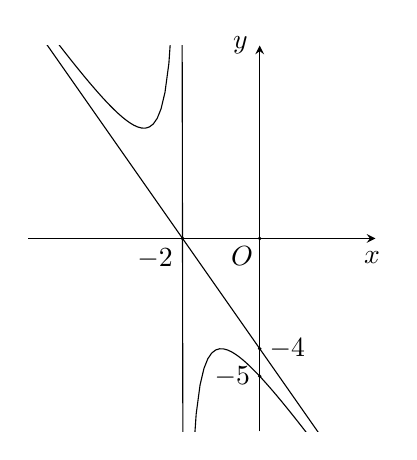
\begin{tikzpicture}[scale=.7,line cap=butt,line join=miter,>=stealth,x=.7cm,y=.5cm]
            \draw[->] (-6,0)--(3,0)
            node[shift={(-100:7pt)},font=\normalsize]{$x$};
            \draw[->] (0,-7)--(0,7)
            node[shift={(180:7pt)},font=\normalsize]{$y$};
            \draw (0,0) node[shift={(225:9pt)},font=\normalsize]{$O$};
            \tikzset{declare function={f(\x)=-2*(\x)-4-2/((\x)+2);}}
            \fill (-2,0) circle(1pt) node[below left]{$-2$}
            (0,0) circle(1pt) 
            (0,-4) circle(1pt) node[right]{$-4$}
            (0,-5) circle(1pt) node[left]{$-5$}
            ;
            \begin{scope}
                \clip (-6,-7) rectangle (3,7);
                \draw[samples=100] plot[domain=-7:3] (\x, {f(\x)});
            \end{scope}
            \tikzset{declare function={g(\x)=-2*(\x)-4;}}
            \begin{scope}
                \clip (-6,-7) rectangle (3,7);
                \draw[samples=100] plot[domain=-7:3] (\x, {g(\x)});
            \end{scope}
    \end{tikzpicture}}
%    \loigiai
%    {\begin{itemchoice}
%            \itemch \textbf{Đúng}. Từ hình vẽ ta thấy đồ thị hàm số đã cho có tiệm cận đứng là đường thẳng $x=-2$, suy ra $d=2$.
%            \itemch \textbf{Đúng}. Đồ thị hàm số đã cho có tiệm cận xiên là đường thẳng $y=ax+b$ đi qua các điểm $\left(0;-4\right)$ và $\left(-2; 0\right)$ nên $b=-4$, $a=-2$.
%            \itemch \textbf{Sai}. Tiệm cận xiên của đồ thị hàm số là đường thẳng $y=-2x-4$.
%            \itemch \textbf{Đúng}. Đồ thị hàm số $y=-2x-4+\dfrac{c}{x+2}$ đi qua điểm $\left(0;-5\right)$ nên ta có $-5=-4+\dfrac{c}{2} \Rightarrow c=-2$.\\
%            Vậy hàm số đã cho là $y=-2x-4-\dfrac{2}{x+2}$.
%        \end{itemchoice}
%    }
    \dotlineEX{1}
\end{ex}
\begin{ex}[TN2025-0101]%%[0D7V2-7]
    Nếu một doanh nghiệp sản xuất $x$ sản phẩm trong một tháng ($x \in \mathbb{N}^*$; $1 \leq x \leq 4\,500$) thì doanh thu nhận được khi bán hết số sản phẩm đó là $F(x)= -0{,}01x^2 + 300x$ (nghìn đồng), trong khi chi phí sản xuất bình quân cho mỗi sản phẩm là $G(x)=\dfrac{30\,000}{x} + 200$ (nghìn đồng). Giả sử số sản phẩm sản xuất ra luôn được bán hết. Trong một tháng, doanh nghiệp đó cần sản xuất ít nhất bao nhiêu sản phẩm để lợi nhuận thu được lớn hơn $100$ triệu đồng?
    \shortans{$1\,536$}
    \loigiai{
        Tổng chi phí sản xuất $C(x)$ cho $x$ sản phẩm là
        $$C(x) = x \cdot G(x) = x \left( \dfrac{30\,000}{x} + 200 \right) = 30\,000 + 200x\text{ (nghìn đồng)}.$$
        Lợi nhuận $P(x)$ thu được khi bán $x$ sản phẩm là 
        \begin{eqnarray*}
            P(x) &=& F(x) - C(x)\\
            &=& \left(-0{,}01x^2 + 300x\right) - (30\,000 + 200x)\\
            &=& -0{,}01x^2 + 100x - 30\,000 \text{ (nghìn đồng)}.
        \end{eqnarray*}
        Doanh nghiệp muốn lợi nhuận thu được lớn hơn $100$ triệu đồng, nên ta có
        \begin{eqnarray*}
            &&P(x)> 100\,000\\
            &\Leftrightarrow&-0{,}01x^2 + 100x - 30\,000>100\,000\\
            &\Leftrightarrow&-0{,}01x^2 +100x - 130\,000>0\\
            &\Leftrightarrow&1\, 535{,}9<x<8\, 464{,}1.
        \end{eqnarray*}
        Kết hợp với điều kiện $x\in \mathbb{N}^*$ và $1\le x\le 4\,500$, suy ra $1\,536\le x\le 4\,500$.\\
        Vậy doanh nghiệp cần sản xuất ít nhất $1\,536$ sản phẩm để lợi nhuận thu được lớn hơn $100$ triệu đồng.
    }
    \dotlineEX{3}
\end{ex}
\begin{ex}[THPT Huế]%[2D1C3-6]
    Một cơ sở sản xuất khăn đang bán mỗi chiếc khăn với giá $30\,000$ đồng một chiếc và mỗi tháng cơ sở bán được trung bình $3\,000$ chiếc khăn. Cơ sở sản xuất đang có kế hoạch tăng giá bán để có lợi nhuận tốt hơn. Sau khi tham khảo thị trường, người quản lý thấy rằng nếu từ mức giá $30\,000$ đồng mà cứ tăng giá thêm $1\,000$ đồng thì mỗi tháng sẽ bán ít hơn $100$ chiếc. Biết vốn sản xuất một chiếc khăn không thay đổi là $18\,000$ đồng. Để đạt lợi nhuận lớn nhất thì mỗi chiếc khăn cần bán với giá bao nhiêu nghìn đồng?
    \shortans{$39$}
    \loigiai{
        Vì cứ tăng giá bán thêm $1$ (nghìn đồng) thì số khăn bán ra giảm $100$ chiếc nên tăng $x$ (nghìn đồng) thì số khăn bán ra giảm $100x$ chiếc.\\
        Do dó tổng số khăn bán ra mỗi tháng là $3\,000 - 100x$ (chiếc).\\
        Lúc đầu bán với giá $30$ (nghìn đồng), mỗi chiếc khăn có lãi $12$ (nghìn đồng). Sau khi tăng giá, mỗi chiếc khăn thu được số lãi là $12 + x$ (nghìn đồng).\\
        Do đó tổng số lợi nhuận một tháng thu được sau khi tăng giá là $f(x) = \left(3\,000 - 100x \right)\left(12 + x \right)$ trên $\left(0; +\infty \right)$.\\
        Ta có $f(x) = -100x^2 + 1\,800x + 36\,000$.\\
        Suy ra $f'(x) = -200x + 1\,800$.\\
        Xét $f'(x) = 0 \Leftrightarrow -200x + 1\,800 = 0 \Leftrightarrow x = 9$.\\
        Ta có bảng biến thiên
        \begin{center}
            
\begin{tikzpicture}[font=\normalsize]
                %dòng khai báo
                \tkzTabInit[nocadre=true,lgt=1.2,espcl=3,deltacl=0.6]
                {$x$/0.75, $f(x)$/2}
                {$ 0 $, $ 9 $, $ +\infty $}
                %dòng biến thiên
                \tkzTabVar{-/$36000$,+/$ 44100 $,-/$-\infty$}
            \end{tikzpicture}
        \end{center}
        Từ bảng biến thiên của hàm số $f(x)$ trên $\left(0; +\infty \right)$ ta thấy hàm số đạt giá trị lớn nhất khi $x = 9$.\\
        Như vậy, để thu được lợi nhuận cao nhất thì cơ sở sản xuất cần tăng giá bán mỗi chiếc khăn là $9\,000$ đồng, tức là mỗi chiếc khăn bán với giá mới là $39\,000$ đồng.
    }
    \dotlineEX{4}
\end{ex}
\begin{ex}[CHUYÊN PHAN BỘI CHÂU]%[2D1V3-6]
    Chi phí về nhiên liệu của một con tàu được chia làm hai phần. Phần chi phí thứ nhất không phụ thuộc vào tốc độ tàu và bằng $480$ nghìn đồng mỗi giờ. Chi phí phần thứ hai trên $1$\,km đường tỉ lệ thuận với lập phương của tốc độ tàu, khi tốc độ bằng $20$\,km/h thì chi phí phần thứ hai bằng $100$ nghìn đồng mỗi giờ. Giả sử con tàu đó luôn giữ nguyên tốc độ di chuyển, để tổng chi phí nhiên liệu trên $1$\,km đường là nhỏ nhất thì tốc độ của con tàu đó bằng bao nhiêu km/h? (làm tròn kết quả đến hàng phần chục).
    \shortans{$22{,}5$}
    \loigiai{
        Gọi $x$ (km/h) là tốc độ của tàu. Thời gian tàu chạy quãng đường $1$ km là $\dfrac{1}{x}$ (giờ).\\
        Chi phí tiền nhiên liệu phần thứ nhất cho quãng đường $1$ km là $\dfrac{480}{x}$ (nghìn đồng).\\
        Gọi $y$ (nghìn đồng) là chi phí nhiên liệu phần thứ hai cho quãng đường $1$ km ứng với tốc độ $x$.\\
        Ta có $y$ tỉ lệ thuận với lập phương tốc độ nên $y=kx^3$ với $k>0$\\
        Khi tốc độ $x=20$ (km/h) thì thời gian tàu chạy $1$ km là $\dfrac{1}{20}$ (giờ) nên chi phí phần thứ $2$ cho quãng đường $1$ km là $\dfrac{1}{20}\cdot100=5$ (nghìn đồng).\\
        Suy ra $5=k\cdot 20^3$ nên $k=\dfrac{1}{1\,600}$, do đó $y=\dfrac{1}{1\,600}x^3$.\\
        Vậy tổng chi phí tiền nhiên liệu cho $1$\,km đường là $$P(x)=\dfrac{480}{x}+\dfrac{x^3}{1\,600}.$$
        Bài toán trở thành tìm $x$ để $P(x)$ nhỏ nhất.\\
        Ta có $P'(x)=-\dfrac{480}{x^2}+\dfrac{3x^2}{1600}=0\Leftrightarrow x=4\sqrt[4]{1\,000}$.\\
        Vậy để tổng chi phí trên $1$ km đường nhỏ nhất thì vận tốc của tàu là $x=4\sqrt[4]{1\,000}\approx 22{,}5$ (km/h).
    }
    \dotlineEX{3}
\end{ex}
\begin{ex}[SỞ YÊN BÁI]%[2D1V3-6]
    Nhà máy $A$ chuyên sản xuất một loại sản phẩm cung cấp cho nhà máy $B$. Hai nhà máy thỏa thuận rằng, hàng tháng nhà máy $A$ cung cấp cho nhà máy $B$ số lượng sản phẩm theo đơn đặt hàng của $B$ (tối đa $100$ tấn sản phẩm). Nếu số lượng đặt hàng là $x$ tấn sản phẩm thì giá bán cho mỗi tấn sản phẩm là $P(x)=45-0{,}001x^2$ (triệu đồng). Chi phí để $A$ sản xuất $x$ tấn sản phẩm trong một tháng gồm $100$ triệu đồng chi phí cố định và $30$ triệu đồng cho mỗi tấn sản phẩm. Nhà máy $A$ cần bán cho nhà máy $B$ bao nhiêu tấn sản phẩm mỗi tháng để lợi nhuận thu được lớn nhất? (kết quả làm tròn đến hàng phần chục).
    \shortans{$70{,}7$}
    \loigiai{
        Tổng chi phí cho $x$ tấn sản phẩm là $C(x)=100+30x$, $0<x\le 100$. \\
        Tổng doanh thu khi bán $x$ tấn sản phẩm là $x\cdot P(x)=x\cdot \left(45-0{,}001x^2\right)=45x-0{,}001x^3$.\\
        Lợi nhuận thu về khi bán hết $x$ tấn sản phẩm là $L(x)=x\cdot P(x)-C(x)=-0{,}001x^3+15x-55$. \\
        Ta có $L'(x)=-0{,}003x^2+15=0
        \Leftrightarrow \hoac{&x=50\sqrt{2}\approx 70{,}71 \text{ (nhận)} 
            \Rightarrow L\approx 652 \\&x=-50\sqrt{2} \text{ (loại)}.}$\\
        Bảng biến thiên
        \begin{center}	
            \begin{tikzpicture}[line join=round,>=stealth]
                \def\myltespcl{3}\def\myltlgt{2}\def\myltdeltacl{0.5}
                \def\myltx{0.7}\def\mylta{0.7}\def\myltb{2.1}\def\myltc{\myltb/3}
                \path(\myltlgt/2,-\myltx/2) node {$x$}(\myltlgt/2,-\myltx-\mylta/2) node {$y'$}(\myltlgt/2,-\myltx-\mylta-\myltb/2) node {$y$};
                \draw(0,-\myltx)--(\myltlgt+2*\myltespcl+2*\myltdeltacl,-\myltx)(0,-\myltx-\mylta)--(\myltlgt+2*\myltespcl+2*\myltdeltacl,-\myltx-\mylta)(\myltlgt,0)--(\myltlgt,-\myltx-\mylta-\myltb);
                \path(\myltlgt+\myltdeltacl,-\myltx/2) node {$0$};
                \path(\myltlgt+\myltdeltacl+0.5*\myltespcl,-\myltx-\mylta/2) node {$+$};
                \path(\myltlgt+\myltdeltacl+\myltespcl,-\myltx/2) node {$50\sqrt 2$};
                \path(\myltlgt+\myltdeltacl+1.5*\myltespcl,-\myltx-\mylta/2) node {$-$};
                \path(\myltlgt+\myltdeltacl+2*\myltespcl,-\myltx/2) node {$+\infty$};
                \path(\myltlgt+\myltdeltacl+\myltespcl,-\myltx-\mylta/2) node {$0$};
                \node (nmylta) at (\myltlgt+\myltdeltacl,-\myltx-\mylta-2.5*\myltc) {$0$};
                \node (nmyltb) at (\myltlgt+\myltdeltacl+\myltespcl,-\myltx-\mylta-0.5*\myltc) {$652$};
                \node (nmyltc) at (\myltlgt+\myltdeltacl+2*\myltespcl,-\myltx-\mylta-2.5*\myltc) {$-\infty$};
                \draw[->] (nmylta)--(nmyltb);
                \draw[->] (nmyltb)--(nmyltc);
            \end{tikzpicture}
        \end{center}
        Vậy nhà máy $A$ cần bán $70{,}7$ tấn sản phẩm cho nhà máy $B$ để lợi nhuận thu về tối đa.
    }
    \dotlineEX{2}
\end{ex}
%\begin{ex}[CHUYÊN PHAN BỘI CHÂU - HÀ TỈNH]%[2D1V2-7]
%    Doanh số (tính bằng số sản phẩm) của một sản phẩm mới (trong vòng một số năm nhất định) được mô hình hóa bằng hàm số $f(t) = \dfrac{24000}{1 + 6e^{-t}},\ t \geq 0$, trong đó thời gian $t$ được tính bằng năm, kể từ khi phát hành sản phẩm mới. Khi đó, đạo hàm $f'(t)$ sẽ biểu thị tốc độ bán hàng. Tốc độ bán hàng lớn nhất đạt được khi $t = \ln a$.  
%    Tìm $a$?
%    \shortans{$6$}
%    \loigiai
%    {
%        Hàm số biểu thị tốc độ bán hàng là
%        \begin{equation*}
%            g(t) = f'(t) = \dfrac{-24000 \cdot (-6e^{-t})}{(1 + 6e^{-t})^2}
%            = \dfrac{144000e^{-t}}{(1 + 6e^{-t})^2},\quad \text{với } t \geq 0.
%        \end{equation*}
%        Ta có
%        \begin{equation*}
%            g'(t) = \dfrac{-144000e^{-t} \cdot (1 + 6e^{-t})^2 - 2 \cdot (1 + 6e^{-t}) \cdot (-6e^{-t}) \cdot 144000e^{-t}}{(1 + 6e^{-t})^4} = -144000 \cdot \dfrac{(e^{t} -6)e^{t}}{( e^{t}+6)^3}
%        \end{equation*}
%        Xét $g'(t)=0\Leftrightarrow t=\ln 6$.\\
%        Vậy tốc độ bán hàng lớn nhất đạt được khi $t = \ln 6$.  
%    }
%    \dotlineEX{2}
%\end{ex}
\begin{ex}[CHUYÊN LƯƠNG THẾ VINH]%[0D1N1-5]
    Nhà máy $A$ chuyên sản xuất một loại sản phẩm cho nhà máy $B$. Hai nhà máy thỏa thuận rằng hằng tháng nhà máy $A$ cung cấp cho nhà máy $B$ sản phẩm đó theo đơn đặt hàng của nhà máy $B$ với số lượng tối đa là $100$ tấn sản phẩm. Nếu số lượng đặt hàng là $x$ tấn sản phẩm thì giá bán của mỗi tấn sản phẩm là $P(x)=45-0,001 x^2$ (triệu đồng). Chi phí để nhà máy $A$ sản xuất $x$ tấn sản phẩm trong một tháng là $C(x)=100+30 x$ (triệu đồng), gồm $100$ triệu đồng chi phí cố định và $30$ triệu đồng cho mỗi tấn sản phẩm. Hỏi nhà máy $A$ bán cho nhà máy $B$ bao nhiêu tấn sản phẩm mỗi tháng thì thu được lợi nhuận lớn nhất? (kết quả làm tròn đến một chữ số thập phân)
    \shortans{$70{,}7$}
    \loigiai
    {Nếu mỗi tháng nhà máy $A$ bán cho nhà máy $B$ $x$ tấn sản phẩm thì lợi nhuận của nhà máy $A$ thu được là
        $$
        x\left(45-0{,}001 x^2\right)-(100+30 x)=-0{,}001 x^3+15 x-100.
        $$
        Xét hàm số $f(x)=-0{,}001 x^3+15 x-100$ với $x \in[0; 100]$.\\
        Ta tìm giá trị lớn nhất của $f(x)$.\\
        Ta có $f'(x)=-0{,}003 x^2+15$; $f^{\prime}(x)=0 \Leftrightarrow x=50 \sqrt{2}$ (do $x \in[0; 100]$).\\
        Vì $f(0)=-100$, $f(50 \sqrt{2}) \approx 607$, $f(100)=400$ nên $f(x)$ lớn nhất khi $x=50 \sqrt{2} \approx 70{,}7$.
    }
    \dotlineEX{2}
\end{ex}

\begin{ex}[SỞ BÌNH PHƯỚC]%[2D1V3-6] 
    Một doanh nghiệp kinh doanh một loại sản phẩm $T$ được sản xuất trong nước. Qua nghiên cứu thấy rằng nếu chi phí sản xuất mỗi sản phẩm $T$ là $x$ (\$) thì số sản phẩm $T$ các nhà máy sản xuất sẽ là $R(x)=x-200$ và số sản phẩm $T$ mà doanh nghiệp bán được trên thị trường trong nước sẽ là $Q(x)=4\,200-x $. Số sản phẩm còn dư doanh nghiệp xuất khẩu ra thị trường quốc tế với giá bán mỗi sản phẩm ổn định trên thị trường quốc tế là $x_0=3\,200$ (\$). Nhà nước đánh thuế trên mỗi sản phẩm xuất khẩu là $a$ (\$) và luôn đảm bảo tỉ lệ giữa lãi xuất khẩu của doanh nghiệp và thuế thu được của nhà nước tương ứng là $4:1$. Hãy xác định giá trị của $a$ biết lãi mà doanh nghiệp thu được do xuất khẩu là nhiều nhất.
    \shortans[oly]{100}
    \loigiai{
        Điều kiện $R(x)=x-200 > 0$; $Q(x)=4\,200-x > 0$ nên $200 < x < 4\,200$.\\
        Số sản phẩm xuất khẩu là $R(x)-Q(x)=x-200-(4200-x)=2x-4400$.\\		
        Lãi xuất khẩu của doanh nghiệp là
        $$L(x)=\left(R(x)-Q(x)\right)(3\,200-x-a)=(2x-4\,400)(3\,200-x-a).$$		
        Thuế thu được của nhà nước là $T(x)=(2x-4\,400)a$.\\
        Ta có\\
        $L(x):T(x)=4:1$, suy ra $(2x-4\,400)(3\,200-x-a)=4(2x-4\,400)a $$ \Rightarrow a=\dfrac{3\,200-x}{5}$.\\		
        Khi đó\\
        $L(x)=(2x-4\,400)\left(3\,200-x-\dfrac{3\,200-x}{5} \right)=(2x-4\,400)\dfrac{12\,800-4x}{5}=\dfrac{1}{5} \left(-8x^2+43\,200x-56\,320\,000\right)$.\\	
        Ta cần tìm $x$ để $L(x)$ đạt giá trị lớn nhất.\\
        Ta có $L'(x)=\dfrac{1}{5} (-16x+43\,200)=0\Leftrightarrow x=2\,700\in (200; 4200)$.\\
        Lập bảng biến thiên ta có 		
        \begin{center}
            
\begin{tikzpicture}
                \tkzTabInit[nocadre=false,lgt=1.5,espcl=2,deltacl=0.6]
                {$x$/0.7,$L'$/0.7,$L$/2}
                {$200$,$2\,700$,$4\,200$}
                \tkzTabLine{,+,0,-,}
                \tkzTabVar{-/$~$,+/$L(2\,700)$,-/$~$}
            \end{tikzpicture}
        \end{center}
        Suy ra $L(x)$ đạt giá trị lớn nhất khi $x=2\,700$.\\		
        Suy ra $a=\dfrac{3\,200-2\,700}{5}=100$.
    }
    \dotlineEX{2}
\end{ex}

\begin{ex}[CHUYÊ LÊ KHIẾT]%[2D1H3-6]
    \immini[thm]{
        Hai thành phố ở hai vị trí $A$ và $B$ cách nhau một con sông. Người ta xây dựng một cây cầu bắc qua sông biết rằng vị trí $A$ cách con sông một khoảng là $4$ km, vị trí $B$ cách con sông một khoảng là $6$ km, $HE+KF=20$ km và độ dài $EF$ không đổi. Hỏi độ dài $EH$ là bao nhiêu km để đường đi từ thành phố $A$ đến thành phố $B$ là ngắn nhất? 
        \shortans{$8$} 
    }{
        \begin{tikzpicture}
            \path    
            (0,0) coordinate (A) 
            (2,0) coordinate (H) 
            (2,-1) coordinate (E)
            (5,-1) coordinate (F)
            (5,-2) coordinate (K)
            (8,-2) coordinate (B)
            ; 
            \fill[fill=green!30] (2,1.5) -- (2,-3.5) -- (5,-3.5) -- (5,1.5) -- cycle;
            %\shade[ball color=blue!20] (M) circle (1.4);
            \draw (H)--(A)node[pos=0.5, above,scale=.8]{$4$ km}--(E)--(F)--(B)--(K)node[pos=0.5, below,scale=.8]{$6$ km} (2,1.5) -- (2,-3.5) (5,-3.5) -- (5,1.5); 
            \foreach \x / \goc in {A/90,B/-90,E/-130,F/60,H/120,K/-40} \fill (\x) circle (1pt) ($(\x)+(\goc:3mm)$) node[scale=.8] {$\x$};
        \end{tikzpicture} 
    }
    \loigiai{
        Đặt $HE=x,\,\left( 0\le x\le 20 \right) \Rightarrow  KF=20-x \Rightarrow  AE=\sqrt{16+x^2}$, $FB=\sqrt{36+\left( 20-x \right)^2}$.\\
        Đường đi từ thành phố $A$ đến thành phố $B$ là $AE+EF+KB$.\\
        Để đường đi từ thành phố $A$ đến thành phố $B$ là ngắn nhất thì $AE+KB$ đạt giá trị nhỏ nhất.\\
        Đặt $f\left( x \right)=AE+KB=\sqrt{16+x^2}+\sqrt{36+\left( 20-x \right)^2}$.\\
        Ta có $f'\left( x \right)=\dfrac{x}{\sqrt{16+x^2}}-\dfrac{20-x}{\sqrt{36+\left( 20-x \right)^2}}$.\\
        Suy ra $f'\left( x \right)=0 \Leftrightarrow \dfrac{x}{\sqrt{16+x^2}}-\dfrac{20-x}{\sqrt{36+\left( 20-x \right)^2}}=0$
        $$\Leftrightarrow \dfrac{x}{\sqrt{16+x^2}}=\dfrac{20-x}{\sqrt{36+\left( 20-x \right)^2}} \Rightarrow \hoac{& x=8 ~\left( \text{thỏa mãn} \right) \\ 
            & x=-40.~\left( \text{loại} \right)}$$
        Bảng biến thiên
        \begin{center}
            
\begin{tikzpicture}
                \tkzTabInit[nocadre,lgt=1.5,espcl=2.5,deltacl=.5]
                {$x$ /.7, $f’(x)$ /.7,$f(x)$ /2}
                {$0$ , $8$, $20$}
                \tkzTabLine{,-,z,+,}
                \tkzTabVar{+/$ $ ,-/ $ $ ,+/$ $}
            \end{tikzpicture}
        \end{center}
        Vậy độ dài $EH=8$ km thì đường đi từ thành phố $A$ đến thành phố $B$ là ngắn nhất.
    }
    \dotlineEX{2}
\end{ex}

\begin{ex}[SỞ HẬU GIANG]%[2D1V3-6]
    \immini[thm]{
      Anh Tí muốn chèo thuyền từ vị trí $A$ đến vị trí $B$ về phía hạ lưu bờ đối diện, càng nhanh càng tốt, trên một bờ sông thẳng rộng $3$km (như hình vẽ). Tí có thể chèo thuyền của mình trực tiếp qua sông để đến vị trí $C$ và sau đó chạy đến vị trí $B$, hay có thể chèo trực tiếp từ vị trí $A$ đến vị trí $B$, hoặc anh ta có thể chèo đến một vị trí $D$ ở giữa $C$ và $B$ và sau đó chạy đến $B$. Biết anh ấy có thể chèo thuyền với tốc độ $6$km/h, chạy với tốc độ $8$km/h và quãng đường $BC=8$km. Biết tốc độ của dòng nước là không đáng kể có với tốc độ chèo thuyền của anh Tí. Khoảng thời gian để anh Tí đến $B$ là bao nhiêu phút? (Kết quả làm tròn đến hàng đơn vị)
    }
    {
        \begin{tikzpicture}[scale=1, font=\footnotesize, line join=round, line cap=round, >=stealth]
            \fill[blue!20]
            (0,0.5)--(3,0.5)--(3,-3.5)--(0,-3.5)--cycle
            ;
            \path 
            (0,0) coordinate (A) node[left]{$A$}
            (3,0) coordinate (C) node[right]{$C$}
            (3,-2) coordinate (D) node[right]{$D$}
            (3,-3) coordinate (B)node[right]{$B$}
            ;
            
            \draw[->] (A)--(C) node[above, midway]{$3$km} (A)--(D) (A)--(B)
            ;
            \draw[<->] ($(C)+(0:0.5)$)--($(B)+(0:0.5)$) node[midway,above,rotate=-90]{$8$km};
        \end{tikzpicture}
    }
    \shortans[0]{80}
    \loigiai{
        Gọi $x=CD$, khi đó $AD=\sqrt{AC^2+CD^2}=\sqrt{x^2+9}$ và $BD=8-x$ với $0\le x\le 8$.\\
        Thời gian anh Tí đi từ $A$ đến $B$ là $t(x)=\dfrac{\sqrt{x^2+9}}{6}+\dfrac{8-x}{8}$.\\
        Ta có $t'(x)=\dfrac{1}{6}\cdot \dfrac{x}{\sqrt{x^2+9}}-\dfrac{1}{8}$.\\
        $t'(x)=0
        \Leftrightarrow \dfrac{x}{6\sqrt{x^2+9}}-\dfrac{1}{8}=0
        \Leftrightarrow 3\sqrt{x^2+9}=4x
        \Rightarrow 7x^2=81
        \Rightarrow x=\pm \dfrac{9}{\sqrt{7}}$.\\
        Vì $x\in \left[ 0;8 \right]$ nên $x=\dfrac{9}{\sqrt{7}}$.\\
        Ta có: $t(0)=\dfrac{3}{2}$; $t(8)=\dfrac{\sqrt{73}}{6}$, $t\left( \dfrac{9}{\sqrt{7}} \right)=\dfrac{8+\sqrt{7}}{8}$.\\
        Vậy thời gian ngắn nhất khi $x=\dfrac{9}{\sqrt{7}}$ và $t\left( \dfrac{9}{\sqrt{7}} \right)\approx 1,33\text{ giờ}\approx 80\text{ phút}$.
    }
\end{ex}



\begin{ex}[SỞ VĨNH PHÚC]%[2D1V3-6]
    \immini[thm]{Một khu đất có hình dạng là một nửa hình tròn bán kính $18$ m. Người ta muốn xây dựng một khu vui chơi hình chữ nhật ở bên trong nửa đường tròn đó,biết rằng một cạnh của hình chữ nhật nằm dọc trên đường kính của nửa đường tròn (tham khảo hình vẽ). Tính diện tích lớn nhất của khu vui chơi có thể xây dựng.
    }{
        \begin{tikzpicture}
            \coordinate (M) at (0,0);
            \coordinate (N) at (4,0);
            \coordinate (O) at (1,0);
            \coordinate (C) at ($(O) + (120:3)$);
            \coordinate (D) at ($(O) + (60:3)$);
            \coordinate (A) at ($(C)-(0,2.6)$);
            \coordinate (B) at ($(D)-(0,2.6)$);
            \draw (N) arc (0:180:3cm) (-2,0)--(4,0);
            \draw (A)--(C)--(D)--(B);
            \draw (1,1) node {Khu vui chơi};
        \end{tikzpicture}
    }
    \shortans{$324$}
    \loigiai{
        \begin{center}
            \begin{tikzpicture}[thick]
                \coordinate (M) at (0,0);
                \coordinate (N) at (4,0);
                \coordinate (O) at (1,0);
                \coordinate (C) at ($(O) + (120:3)$);
                \coordinate (D) at ($(O) + (60:3)$);
                \coordinate (A) at ($(C)-(0,2.6)$);
                \coordinate (B) at ($(D)-(0,2.6)$);
                \draw (N) arc (0:180:3cm) (-2,0)--(4,0);
                \draw (A)--(C)--(D)--(B) (O)--(C);
                %Gán nhãn.
                \foreach \x/\y in {O/-90, C/120, D/60, A/-90, B/-90}{\fill (\x) circle(1pt) ($(\x)+(\y:0.3cm)$) node{$\x$};}
            \end{tikzpicture}
        \end{center}
        Gọi $AO=x\Rightarrow AB=2x$, $AC=y$, ($x$, $y>0$).\\
        Khi đó diện tích hình chữ nhật (khu vui chơi) là $S=2x\cdot y$.\\
        Xét tam giác vuông $CAO$ vuông tại $A$, ta có $AO^2+AC^2=OC^2\Leftrightarrow x^2+y^2=18^2$.\\
        Áp dụng bất đẳng thức Cauchy cho $2$ số dương $x$, $y$ ta có $$x^2+y^2\ge 2\cdot\sqrt{x^2y^2}\Leftrightarrow x y\le\dfrac{x^2+y^2}{2}.$$
        Do đó $S=2x y\le 2\cdot\dfrac{x^2+y^2}{2}\Leftrightarrow S\le 18^2$.\\ Dấu \lq\lq$=$\rq\rq\, xảy ra khi $x=y=9\sqrt{2}$.\\
        Vậy giá trị lớn nhất của diện tích khu vui chơi là $324$ (m$^2$).
    }
    \dotlineEX{3}
\end{ex}
\begin{ex}%[1H8V7-9]
    \immini[thm]{
        Từ một tấm bìa mỏng hình vuông cạnh $6$ dm, bạn Hoa cắt bỏ bốn tam giác cân bằng nhau có cạnh đáy là cạnh của hình vuông ban đầu và đỉnh là đỉnh của một hình vuông nhỏ phía trong rồi gập lên, ghép lại tạo thành một khối chóp tứ giác đều như hình bên. Thể tích của khối chóp có giá trị lớn nhất bằng bao nhiêu decimét khối (làm tròn kết quả đến hàng phần mười)?
        \shortans{$7{,}3$}
    }
    {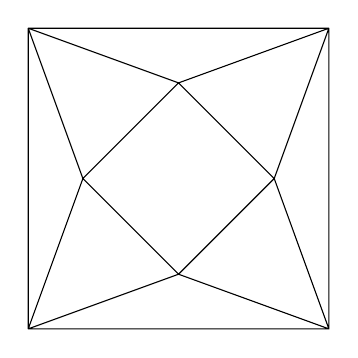
\begin{tikzpicture}[scale=0.9, font=\small, line join=round, line cap=round, >=stealth]
            \def\R{3} \def\r{0.45*\R}
            \path (0,0) coordinate(O);
            \foreach \i [count=\j from 0] in {B,A,D,C} \path ({90*\j+45}:\R) coordinate(\i);
            \foreach \t [count=\k from 0] in {N,M,Q,P} \path ({90*\k}:\r) coordinate(\t);
            \draw (A)--(B)--(C)--(D)--cycle
            (M)--(N)--(P)--(Q)--cycle
            (A)--(M)--(B)--(N)--(C)--(P)--(D)--(Q)--(A);
    \end{tikzpicture}}
    \loigiai
    {Giả sử miếng bìa là hình vuông $ABCD$, đáy của hình chóp tứ giác đều là hình vuông $MNPQ$ tâm $O$ có cạnh bằng $x$ dm ($0<x<6 \sqrt{2}$) như hình vẽ. Gọi $H$, $K$ lần lượt là trung điểm của $MQ$ và $NP$.
        \begin{center}
            \begin{tikzpicture}[scale=1, font=\small, line join=round, line cap=round, >=stealth]
                \def\R{3} \def\r{0.45*\R}
                \path (0,0) coordinate(O);
                \foreach \i [count=\j from 0] in {B,A,D,C} \path ({90*\j+45}:\R) coordinate(\i);
                \foreach \t [count=\k from 0] in {N,M,Q,P} \path ({90*\k}:\r) coordinate(\t);
                \path ($(Q)!1/2!(M)$) coordinate(H)
                ($(P)!1/2!(N)$) coordinate(K);
                \draw (A)--(B)node[midway, above]{$6$ dm} --(C)--(D)--cycle
                (M)--(N)node[midway, sloped, above]{$x$ dm} --(P)--(Q)--cycle
                (A)--(M)--(B)--(N)--(C)--(P)--(D)--(Q)--(A)
                (A)--(C);
                \foreach \p/\q in {A/135, B/45, C/-45, D/225, M/90, N/0, P/-90, Q/180, O/45, H/90, K/-90} {\fill (\p) node[shift={(\q:0.3)}]{$\p$} circle(1pt);}
            \end{tikzpicture}
            \hspace*{1cm}
            \begin{tikzpicture}[scale=1, font=\small,line join=round, line cap=round, >=stealth]
                \def\h{3}
                \path (0,0) coordinate (N)
                (-1.7,-1.2) coordinate (P)
                ++(4,0) coordinate (Q)
                ($(N)+(Q)-(P)$) coordinate(M)
                ($(M)!1/2!(P)$) coordinate(O)
                ++(0,\h) coordinate(A)
                ($(M)!1/2!(Q)$) coordinate(H)
                ($(N)!1/2!(P)$) coordinate(K);
                \draw (A)--(P)--(Q)--(M)--(A)--(Q) (A)--(H);
                \draw[dashed] (A)--(N)--(P) (N)--(M) (H)--(K) (A)--(O);
                \foreach \diem/\pos in {A/90, N/160, P/-100, Q/-80, M/0, O/-90, K/-90, H/-70} \fill (\diem) node[shift={(\pos:0.3)}] {$\diem$} circle(1pt);
                \path pic[draw,angle radius=0.2cm]{right angle=A--O--H};
            \end{tikzpicture}
        \end{center}
        Vì $ABCD$ là hình vuông cạnh bằng $6$ dm nên $AC=6\sqrt{2}$ dm, $HK=x$ dm.\\
        Ta có $AH=\dfrac{AC-HK}{2}=3\sqrt{2}-\dfrac{x}{2}$ dm.\\
        Đường cao của hình chóp tứ giác đều là
        \[h=AO=\sqrt{AH^2-OH^2}=\sqrt{\left(3\sqrt{2}-\dfrac{x}{2}\right)^2-\left(\dfrac{x}{2}\right)^2}=\sqrt{18-3\sqrt{2}x}.\]
        Để tạo thành hình chóp thì đường cao $AO>0$, hay $x<3\sqrt{2}$.\\
        Thể tích khối chóp là
        \[V=\dfrac{1}{3}hx^2=\dfrac{1}{3}x^2\sqrt{18-3\sqrt{2}x}=\dfrac{1}{3}\sqrt{x^4\left(18-3\sqrt{2}x\right)}.\]
        Để tìm giá trị lớn nhất của $V$ ta đi tìm giá trị lớn nhất của hàm số
        \allowdisplaybreaks
        \begin{eqnarray*}
            f(x)=x^4\left(18-3\sqrt{2}x\right)\;\text{với}\;0<x<3\sqrt{2}.
        \end{eqnarray*}
        Ta có $f'(x)=x^3\left(-15 \sqrt{2} x+72\right)$, $f'(x)=0$ khi $x=0$ hoặc $x=\dfrac{12 \sqrt{2}}{5}$.\\
        Bảng biến thiên của $f(x)$ như sau
        \begin{center}
            
\begin{tikzpicture}[>=stealth,line join=round,line cap=round,font=\small,scale=1]
                \tkzTabInit[nocadre=false,lgt=1.2,espcl=3.5,deltacl=.55]
                {$x$/0.7, $f'(x)$/0.7, $f(x)$/2.5}
                {$0$,$\dfrac{12\sqrt{2}}{5}$,$3\sqrt{2}$}
                \tkzTabLine{$0$,+,0,-,}
                \tkzTabVar{-/$0$,+/$f\left(\dfrac{12\sqrt{2}}{5}\right)$,-/$0$}
            \end{tikzpicture}
        \end{center}
        Từ bảng biến thiên ta có $\max\limits_{(0; 3 \sqrt{2})}f(x)=f\left(\dfrac{12 \sqrt{2}}{5}\right)\approx 477{,}76$.\\
        Vậy thể tích của khối chóp có giá trị lớn nhất bằng
        \allowdisplaybreaks
        \begin{eqnarray*}
            V_{\max}\approx\dfrac{1}{3}\sqrt{477{,}76}\approx7{,}3\,\left(\text{dm}^3\right).
        \end{eqnarray*}
    }
    \dotlineEX{5}
\end{ex}

\begin{ex}%[1H8C7-9]
    Cho một tấm nhôm hình lục giác đều cạnh $90$ cm. Người ta cắt ở mỗi đỉnh của tấm nhôm hai hình tam giác vuông bằng nhau, biết cạnh góc vuông nhỏ bằng $x$ cm (cắt phần tô đậm của tấm nhôm) rồi gập tấm nhôm như hình vẽ để được một hình lăng trụ lục giác đều không có nắp. Tìm $x$ để thể tích của khối lăng trụ lục giác đều trên là lớn nhất. ({\it kết quả làm tròn đến hàng đơn vị}) \shortans{15}
    \begin{center}
        \begin{tikzpicture}
            \pgfmathsetmacro\n{6} % Số cạnh
            \pgfmathsetmacro\r{2} % Bán kính
            \pgfmathsetmacro{\goc}{360/\n}
            \pgfmathsetmacro{\nn}{\n-1}
            \path (0,0) coordinate (O);
            \foreach \x in {0,...,\nn}
            {
                \pgfmathsetmacro{\xx}{int(\x+1)}
                \path[fill=black] ($(O)+(\goc*\x:\r)$) coordinate (A\xx) circle (1pt)node[shift={(\goc*\x:9pt)}]{};
                \path ($(O)!1/2!(A\xx)$) coordinate (a\xx);
                \draw[rotate=\goc*\x] (0:\r)--(\goc:\r);
                \draw (O)--(A\xx);
            }
            \path
            (A6) coordinate (A0)
            (A1) coordinate (A7)
            ;
            \foreach \x in {1,...,\n}
            {
                \pgfmathsetmacro{\xx}{int(\x+1)}
                \pgfmathsetmacro{\y}{int(\x-1)}
                \path[fill=black]
                ($(A\x)!(a\x)!(A\y)$) coordinate (a\x\y) circle (1pt)
                ($(A\x)!(a\x)!(A\xx)$) coordinate (a\x\xx) circle (1pt)
                ;
                \fill[pattern=north west lines]
                (a\x)--(a\x\y)--(A\x)--(a\x\xx)--cycle;
                \draw[rotate=\goc*\x] (0:\r/2)--(\goc:\r/2);
                \draw (a\x\xx)--(a\x)--(a\x\y);
            }
            \path (current bounding box.south) node[below]{\bfseries Hình 1};
        \end{tikzpicture}
        \begin{tikzpicture}
            \pgfmathsetmacro\n{6} % Số cạnh
            \pgfmathsetmacro\r{2} % Bán kính
            \pgfmathsetmacro{\goc}{360/\n}
            \pgfmathsetmacro{\nn}{\n-1}
            \path (0,0) coordinate (O);
            \foreach \x in {0,...,\nn}
            {
                \pgfmathsetmacro{\xx}{int(\x+1)}
                \path[fill=black] ($(O)+(\goc*\x:\r)$) coordinate (A\xx);
                \path ($(O)!1/2!(A\xx)$) coordinate (a\xx);
                %				\draw[rotate=\goc*\x] (0:\r)--(\goc:\r);
                \draw (O)--(a\xx);
            }
            \path
            (A6) coordinate (A0)
            (A1) coordinate (A7)
            ;
            \foreach \x in {1,...,\n}
            {
                \pgfmathsetmacro{\xx}{int(\x+1)}
                \pgfmathsetmacro{\y}{int(\x-1)}
                \path[fill=black]
                ($(A\x)!(a\x)!(A\y)$) coordinate (a\x\y)
                ($(A\x)!(a\x)!(A\xx)$) coordinate (a\x\xx)
                ;
                %				\draw[rotate=\goc*\x](0:\r)--(\goc:\r);
                %				\fill[white](a\x)--(a\x\y)--(A\x)--(a\x\xx)--cycle;
            }
            \path
            (a1) coordinate (a7)
            (a10) coordinate (a76)
            ;
            \foreach \x in {1,...,\n}
            {
                \pgfmathsetmacro{\xx}{int(\x+1)}
                \pgfmathsetmacro{\y}{int(\x-1)}
                \draw[rotate=\goc*\x] (0:\r/2)--(\goc:\r/2);
                \draw
                (a\x\y)--(a\x)
                (a\x\xx)--(a\x)
                (a\x\xx)--(a\xx\x)
                ;
            }
            \path (current bounding box.south) node[below]{\bfseries Hình 2};
        \end{tikzpicture}
        \begin{tikzpicture}
            \def\h{1.2}
            \path
            (0,0) coordinate (O)
            +(180:1.5) coordinate (C)
            ++(150:1) coordinate (D)
            +(0:1.3) coordinate (E)
            ($(O)!-1!(C)$) coordinate (F)
            ($(O)!-1!(D)$) coordinate (A)
            ($(O)!-1!(E)$) coordinate (B)
            ;
            \foreach \p in {A,B,C,D,E,F}
            \path ($(\p)+(90:\h)$) coordinate (\p');
            \pgfresetboundingbox
            \draw
            (F)--(A)--(B)--(C)
            (D')--(E')--(F')--(A')--(B')--(C')--cycle
            ;
            \foreach \p/\q in {A/A',B/B',C/C',F/F'}
            \draw (\p)--(\q)
            ;
            \draw[dashed] (C)--(D)--(E)--(F) (D)--(D')
            (E)--(E')
            ;
            \path (current bounding box.south) node[below]{\bfseries Hình 3};
        \end{tikzpicture}
    \end{center}
    \loigiai{
        \begin{center}
            \begin{tikzpicture}[font=\small]
                \pgfmathsetmacro\n{6} % Số cạnh
                \pgfmathsetmacro\r{2} % Bán kính
                \pgfmathsetmacro{\goc}{360/\n}
                \pgfmathsetmacro{\nn}{\n-1}
                \path (0,0) coordinate (O);
                \foreach \x in {0,...,\nn}
                {
                    \pgfmathsetmacro{\xx}{int(\x+1)}
                    \path[fill=black] ($(O)+(\goc*\x:\r)$) coordinate (A\xx);
                    \path ($(O)!1/2!(A\xx)$) coordinate (a\xx);
                    %				\draw[rotate=\goc*\x] (0:\r)--(\goc:\r);
                    \draw (O)--(a\xx);
                }
                \path
                (A6) coordinate (A0)
                (A1) coordinate (A7)
                ;
                \foreach \x in {1,...,\n}
                {
                    \pgfmathsetmacro{\xx}{int(\x+1)}
                    \pgfmathsetmacro{\y}{int(\x-1)}
                    \path[fill=black]
                    ($(A\x)!(a\x)!(A\y)$) coordinate (a\x\y)
                    ($(A\x)!(a\x)!(A\xx)$) coordinate (a\x\xx)
                    ;
                    %				\draw[rotate=\goc*\x](0:\r)--(\goc:\r);
                    %				\fill[white](a\x)--(a\x\y)--(A\x)--(a\x\xx)--cycle;
                }
                \path
                (a1) coordinate (a7)
                (a10) coordinate (a76)
                ;
                \foreach \x in {1,...,\n}
                {
                    \pgfmathsetmacro{\xx}{int(\x+1)}
                    \pgfmathsetmacro{\y}{int(\x-1)}
                    \draw[rotate=\goc*\x] (0:\r/2)--(\goc:\r/2);
                    \draw
                    (a\x\y)--(a\x)
                    (a\x\xx)--(a\x)
                    (a\x\xx)--(a\xx\x)
                    ;
                }
                \path
                (a5) node[below left]{$A$}
                (a6) node[below right]{$B$}
                (a56) node[below]{$H$}
                (a65) node[below]{$K$}
                ;
            \end{tikzpicture}
        \end{center}
        Điều kiện $0<x<45$.\\
        Cạnh đáy của lăng trụ lục giác đều $AB=HK=90-2x$\\
        Chiều cao của lăng trụ lục giác đều $HA=MH\cdot\tan 60^\circ=x\sqrt{3}$.\\
        Diện tích đáy của lăng trụ lục giác đều $S_{ABCDEF}=6S_{ABO}=6\cdot\dfrac{\sqrt{3}}{4}{\left(90-2x\right)^2}$.\\
        Thể tích của khối lăng trụ lục giác đều
        \[V(x)=HA\cdot S_{ABCDEF}=\dfrac{9}{2}x{\left(90-2x\right)^2}\,\,
        \text{hay}\,\, V(x)=18x^3-1620x^2+36450x.\]
        Xét hàm số $V(x)=18x^3-1620x^2+36450x$ trên khoảng $\left(0;45\right)$.
        \begin{align*}
            V'(x)=          & 54x^2-3240x+36450 =0          \\
            \Leftrightarrow & \, 54x^2-3240x+36450=0        \\
            \Leftrightarrow & \, \hoac{              & x=15 \\&x=45\ \text{(loại)}. }
        \end{align*}
        Bảng biến thiên
        \begin{center}
            
\begin{tikzpicture}[>=stealth]
                \tkzTabInit[nocadre=false,lgt=1.5,espcl=3,deltacl=1]{$x$/.7 ,$V'(x)$/.7,$V(x)$/2}
                {$0$ , $15$ , $45$}
                \tkzTabLine{ , + , $0$ , - , }
                \tkzTabVar{-/$0$ , +/$243\,000$ , -/$0$}
            \end{tikzpicture}
        \end{center}
        Từ bảng biến thiên ta có $\max\limits_{(0;45)}V(x)=243\,000$ (cm$^3$) khi và chỉ khi $x=15$ cm.\\
        Vậy thể tích của khối lăng trụ lục giác đều lớn nhất khi và chỉ khi $x=15$ cm.
    }
    \dotlineEX{5}
\end{ex}

\begin{ex}%[1H8C7-9]
    Từ một tấm tôn hình vuông cạnh $16$ dm, bác Dũng cắt bỏ bốn phần như nhau ở bốn góc, sau đó bác hàn các mép lại để được một chiếc thùng (không có nắp) là một hình chóp cụt như hình vẽ. Hỏi thùng có thể chứa được nhiều nhất bao nhiêu lít? (Làm tròn kết quả đến hàng đơn vị).\shortans{$351$}
    \begin{center}
        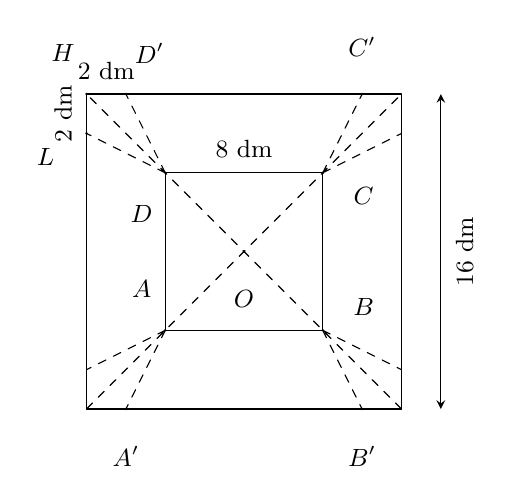
\begin{tikzpicture}[scale=0.5, font=\small, line join=round, line cap=round, >=stealth]
            \path
            (0,0) coordinate (E)
            ++ (0:8) coordinate (F)
            ++ (90:8) coordinate (G)
            ++ (180:8) coordinate (H)
            (2,2) coordinate (A)
            ++ (0:4) coordinate (B)
            ++ (90:4) coordinate (C)
            ++ (180:4) coordinate (D)
            (1,0) coordinate (A')
            (7,0) coordinate (B')
            (8,1) coordinate (J)
            (8,7) coordinate (K)
            (7,8) coordinate (C')
            (1,8) coordinate (D')
            (0,7) coordinate (L)
            (0,1) coordinate (I)
            (4,4) coordinate (O)
            (9,0) coordinate (R)
            (9,8) coordinate (Q)
            ;
            \draw (A)--(B)--(C)--(D)--cycle;
            \draw (E)--(F)--(G)--(H)--cycle;
            \draw[dashed] (E)--(G) (F)--(H) (A)--(A') (A)--(I) (B)--(B') (B)--(J) (C)--(C') (C)--(K) (D)--(D') (D)--(L);
            \draw[<->] (R)--(Q) node[sloped, pos=0.5, shift={(-90:3mm)}] {$16$ dm};
            \draw (H)--(D') node[sloped, pos=0.5, shift={(90:3mm)}] {$2$ dm};
            \draw (L)--(H) node[sloped, pos=0.5, shift={(90:3mm)}] {$2$ dm};
            \draw (D)--(C) node[sloped, pos=0.5, shift={(90:3mm)}] {$8$ dm};
            \foreach \i/\j in {O/-90, A/120, B/30, C/-30, D/-120, A'/-90, B'/-90, C'/90, D'/60, H/120, L/-150}{
                \draw[fill=black] (\i) circle(0.5pt) node[shift={(\j:6mm)}] {$\i$};
            }
        \end{tikzpicture}
        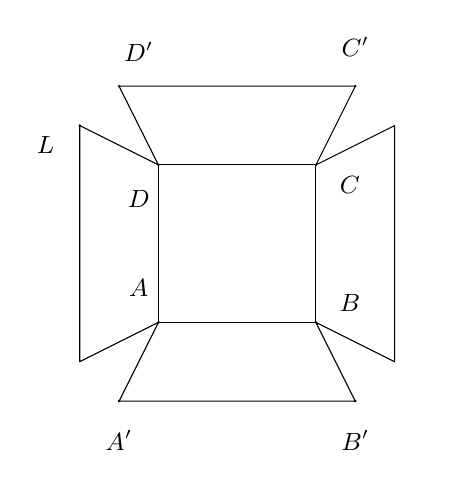
\begin{tikzpicture}[scale=0.5, font=\small, line join=round, line cap=round, >=stealth]
            \path
            (0,0) coordinate (E)
            ++ (0:8) coordinate (F)
            ++ (90:8) coordinate (G)
            ++ (180:8) coordinate (H)
            (2,2) coordinate (A)
            ++ (0:4) coordinate (B)
            ++ (90:4) coordinate (C)
            ++ (180:4) coordinate (D)
            (1,0) coordinate (A')
            (7,0) coordinate (B')
            (8,1) coordinate (J)
            (8,7) coordinate (K)
            (7,8) coordinate (C')
            (1,8) coordinate (D')
            (0,7) coordinate (L)
            (0,1) coordinate (I)
            (4,4) coordinate (O)
            (9,0) coordinate (R)
            (9,8) coordinate (Q)
            ;
            \draw (A)--(B)--(C)--(D)--cycle;
            \draw (A)--(A')--(B')--(B)-- (J)--(K)--(C)-- (C')--(D')--(D)-- (L)--(I)--(A);
            
            \foreach \i/\j in {A/120, B/30, C/-30, D/-120, A'/-90, B'/-90, C'/90, D'/60, L/-150}{
                \draw[fill=black] (\i) circle(0.5pt) node[shift={(\j:5mm)}] {$\i$};
            }
        \end{tikzpicture}
        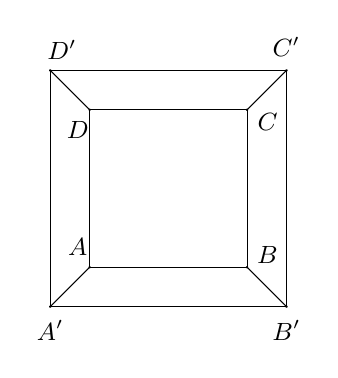
\begin{tikzpicture}[scale=0.5, font=\small, line join=round, line cap=round, >=stealth]
            \path
            (1,1) coordinate (A')
            ++ (0:6) coordinate (B')
            ++ (90:6) coordinate (C')
            ++ (180:6) coordinate (D')
            (2,2) coordinate (A)
            ++ (0:4) coordinate (B)
            ++ (90:4) coordinate (C)
            ++ (180:4) coordinate (D)
            ;
            \draw (A)--(B)--(C)--(D)--cycle;
            \draw (A')--(B')--(C')--(D')--cycle;
            \draw (A)--(A') (B)--(B') (C)--(C') (D)--(D');
            
            \foreach \i/\j in {A/120, B/30, C/-30, D/-120, A'/-90, B'/-90, C'/90, D'/60}{
                \draw[fill=black] (\i) circle(0.5pt) node[shift={(\j:3mm)}] {$\i$};
            }
        \end{tikzpicture}
    \end{center}
    \loigiai
    {
        \begin{center}
            \begin{tikzpicture}[scale=0.7, font=\small, line join=round, line cap=round, >=stealth]
                \path
                (0,0) coordinate (E)
                ++ (0:8) coordinate (F)
                ++ (90:8) coordinate (G)
                ++ (180:8) coordinate (H)
                (2,2) coordinate (A)
                ++ (0:4) coordinate (B)
                ++ (90:4) coordinate (C)
                ++ (180:4) coordinate (D)
                (1,0) coordinate (A')
                (7,0) coordinate (B')
                (8,1) coordinate (J)
                (8,7) coordinate (K)
                (7,8) coordinate (C')
                (1,8) coordinate (D')
                (0,7) coordinate (L)
                (0,1) coordinate (I)
                (4,4) coordinate (O)
                (9,0) coordinate (R)
                (9,8) coordinate (Q)
                (0.5,7.5) coordinate (M)
                ;
                \draw (A)--(B)--(C)--(D)--cycle;
                \draw (E)--(F)--(G)--(H)--cycle;
                \draw[dashed] (E)--(G) (F)--(H) (A)--(A') (A)--(I) (B)--(B') (B)--(J) (C)--(C') (C)--(K) (D)--(D') (D)--(L)--(D');
                \draw[<->] (R)--(Q) node[sloped, pos=0.5, shift={(-90:3mm)}] {$16$ dm};
                \draw (H)--(D') node[sloped, pos=0.5, shift={(90:3mm)}] {$2$ dm};
                \draw (L)--(H) node[sloped, pos=0.5, shift={(90:3mm)}] {$2$ dm};
                \draw (D)--(C) node[sloped, pos=0.5, shift={(90:3mm)}] {$8$ dm};
                \foreach \i/\j in {O/-90, A/120, B/30, C/-30, D/-120, A'/-90, B'/-90, C'/90, D'/60, H/120, L/-150, F/-30}{
                    \draw[fill=black] (\i) circle(0.5pt) node[shift={(\j:5mm)}] {$\i$};
                }
                \draw[fill=black] (M) circle(0.5pt) node[shift={(0:3mm)},font=\scriptsize] {$M$};
                \pic[draw,angle eccentricity=1.8,angle radius=2mm]{right angle=L--M--D};
            \end{tikzpicture}
        \end{center}
        Ta có $HM = MD' = \dfrac{2\sqrt{2}}{2} = \sqrt{2}$.\\
        $HD = \dfrac{HF-DB}{2} = \dfrac{16\sqrt{2} - 8\sqrt{2}}{2} = 4\sqrt{2}$.\\
        $\Rightarrow MD = HD - HM = 4\sqrt{2} - \sqrt{2} = 3\sqrt{2}$.\\
        Áp dụng Định lí Pi-ta-go trong $\triangle D'MD$ vuông tại $M$.\\
        $\Rightarrow D'D = \sqrt{D'M^2 + MD^2} = \sqrt{\sqrt{2}^2 + (3\sqrt{2})^2} = 2\sqrt{5}$.\\
        Vì đây là hình chóp cụt đều nên \\
        $CC' = DD' = AA' = BB' = 2\sqrt{5}$.\\
        Lật ngược hình chóp cụt này lại.\\
        \begin{center}
            \begin{tikzpicture}[scale=1, font=\small, line join=round, line cap=round, >=stealth]
                \path
                (4,7) coordinate (S)
                (0,0) coordinate (A')
                (7,0) coordinate (B')
                (8,3) coordinate (C')
                (1,3) coordinate (D')
                ($(S)!1/3!(A')$) coordinate (A)
                ($(S)!1/3!(B')$) coordinate (B)
                ($(S)!1/3!(C')$) coordinate (C)
                ($(S)!1/3!(D')$) coordinate (D)
                ($(A)!1/2!(C)$) coordinate (O)
                ($(A')!1/2!(C')$) coordinate (O')
                ($(O')!1/3!(C')$) coordinate (E)
                
                ;
                \draw (A)--(B)--(C)--(D)--cycle;
                \draw (D')--(A')--(B')--(C') (A)--(C) (B)--(D);
                \draw[dashed] (A')--(C')--(D')--(B') (O)--(O') (C)--(E);
                \draw (A)--(A') (B)--(B') (C)--(C') (D)--(D');
                \foreach \i/\j in {O/90, O'/-90, A/-170, B/-120, C/30, D/120, A'/-120, B'/-60, C'/0, D'/180, E/-90}{
                    \draw[fill=black] (\i) circle(0.5pt) node[shift={(\j:3mm)}] {$\i$};
                }
                \pic[draw,angle eccentricity=1.8,angle radius=2mm]{right angle=O--O'--C'};
                \pic[draw,angle eccentricity=1.8,angle radius=2mm]{right angle=C--E--C'};
                \draw (C)--(C') node[sloped, pos=0.5, shift={(90:3mm)}] {$2\sqrt{5}$ dm};
                
            \end{tikzpicture}
        \end{center}
        Kẻ $CE \perp A'C'$ tại $E$. Khi đó $O'OCE$ là hình chữ nhật.\\
        $\Rightarrow O'E = OC = \dfrac{AC}{2} = \dfrac{8\sqrt{2}}{2} = 4\sqrt{2}$.\\
        Và $O'C = \dfrac{A'C'}{2} = \dfrac{A'B'\sqrt{2}}{2} = \dfrac{12\sqrt{2}}{2} = 6\sqrt{2}$.\\
        $\Rightarrow EC'=O'C - O'E = 6\sqrt{2} - 4\sqrt{2} = 2\sqrt{2}$.\\
        Áp dụng Định lí Pi-ta-go trong $\triangle CEC'$ vuông tại $E$.\\
        $CE = \sqrt{CC'^2 - EC'^2} = \sqrt{(2\sqrt{5})^2 - (2\sqrt{2})^2} = 2\sqrt{3}$.\\
        Đường cao của hình chóp cụt trên là \\
        $OO' = CE = 2\sqrt{3}$.\\
        Thể tích của hình chóp cụt là\\
        \begin{align*}
            V_{ABCD.A'B'C'D'} & = \dfrac{1}{3}(S_{ABCD} + S_{A'B'C'D'} + \sqrt{S_{ABCD}\cdot S_{A'B'C'D'}})\cdot OO'     \\
            & = \dfrac{1}{3}(8\cdot 8 + 12\cdot 12 + \sqrt{8\cdot 8 \cdot 12 \cdot 12})\cdot 2\sqrt{3} \\
            & = \dfrac{608\sqrt{3}}{3}                                                                 \\
            & \approx 351.
        \end{align*}
        Vậy thể tích của thùng xấp xỉ là $351$ lít.
    }
    \dotlineEX{5}
\end{ex}


\Closesolutionfile{ans}





















